% !TEX encoding = UTF-8 Unicode
\documentclass{pclass}
\usepackage[utf8]{inputenc}
\usepackage{times}
\usepackage{fancyvrb}
\usepackage{longtable}
\usepackage{multirow}
\usepackage{amsmath,amsthm}
\usepackage{graphicx} 
\usepackage{subcaption}
\usepackage{booktabs}
\usepackage{pdflscape}
\usepackage{verbatim}
\usepackage{hyperref}
%\usepackage{ulem}

\theoremstyle{definition}
\newtheorem{problem}{Problema}

\begin{document}
\tipo{Grado}
\titulopro{SIKE: una propuesta de KEM basado en isogenias de curvas elípticas}
\tutor{José Andrés Armario Sampalo}
\departamento{Matemáticas Aplicadas I}
\autores{Alba Ramos Vargas}{{\ }}
\dia{1 de marzo de 2026}
\titulacion{Grado en Ingeniería de Software - Ingeniería Informática}

\hacerportada

	\input{tocdef}
\frontmatter
        
    \cdpchapter{Resumen}

Este proyecto pretende simplificar y acercar a estudiantes de criptografía en el ámbito informático un protocolo diseñado para resistir la computación cuántica conocido como SIKE. A lo largo del documento repasaremos los conceptos matemáticos más importantes en los que se basa el protocolo además de desmigar SIKE y su funcionamiento interno. Finalmente, veremos sin entrar en detalle porqué ya no se considera un protocolo seguro.

Además del documento escrito, el proyecto también cuenta con una interfaz gráfica con un propósito dual: cara al usuario presenta la información de manera dinámica y cara al informático muestra una posible (si bien sencilla) forma de utilización de la implementación de SIKE en Java. La memoria incluye toda la documentación relacionada con el desarrollo técnico de la interfaz.
    \cdpchapter{Abstract}

This projects tries to simplify a protocol designed to bear quantum computing known as SIKE to any cryptography student coming from a computer science domain. In this document we'll review the main mathematical concepts on which the protocol lays in addition to viewing in detail the interior functionning of SIKE. Finally, we'll discuss without too much detail why SIKE is no longer considered secure.

Furthermore, the project also counts with a grpahic interface that serves a dual purpose: on the one hand it relays the information in this document in a dinamic way and in the other hand it shows a computer engineer a possible (if simple) way of using the Java implementation of SIKE. The document thus includes all the information related to the technical development of the interface.

    \tableofcontents
 	\listoftables
 	\listoffigures

 \mainmatter  
    
     \chapter{Introducción}\label{introduccion}

En los últimos años, hemos visto como las tecnologías se disparaban. Desde el establecimiento de Internet y la World Wide Web todo lo informático ha crecido exponencialmente. De teléfonos móviles a teléfonos inteligentes hubo algo más de 20 años\footnote{Tomando de referencia el lanzamiento del DynaTAC\_8000X de Motorola en 1984 y el lanzamiento del primer IPhone de Apple en 2007.}, que es el mismo tiempo que ha pasado de este último a día de hoy.

Últimamente, no hemos dejado de oír de la computación cuántica. Cada poco tiempo se rompe una nueva barrera que previamente se pensaba que estaba a años de ser superada. Es por esto que la criptografía postcuántica es tan importante, en un mundo en el que nuestros datos personales vuelan de una aplicación a otra, proteger la infraestructura digital es no solo un deber sino una necesidad.

El National Institute of Standards and Technology o NIST es un organismo estadounidense perteneciente al ministerio de comercio que desde febrero de 2016, entre otros objetivos, busca establecer unos estándares de seguridad para que podamos mantener la misma seguridad de la que disfrutamos en la actualidad a pesar de este cambio de paradigma.

Debido a que toda migración a esta escala, es decir, a escala mundial, es costosa y lenta, una de las prioridades de la criptografía postcuántica es que todos estos algoritmos deban poder implementarse con los recursos que tenemos hoy en día y los protocolos de redes que utilizamos y, más seguramente, seguiremos utilizando incluso cuando existan los ordenadores cuánticos. Diseñar algoritmos y protocolos que soporten las capacidades de estas máquinas sin poder utilizar su potencia es un verdadero desafío pero no por ello menos importante.

Uno de los protocolos presentados a la convocatoria del NIST es el objeto de este trabajo, Super-singular Isogeny Key Exchange por Luca De Feo, David Jao y Jérôme Plût. SIKE es el único de los protocolos presentados que utiliza la composición de isogenias de curvas elípticas como base matemática de su funcionamiento.

SIKE fue parte de este proceso desde la primera ronda del NIST en diciembre de 2017 hasta la tercera que se cerró en julio de 2022. Sin embargo, poco después se descubriría un ataque efectivo sobre el protocolo que se formalizaría el año siguiente. Debido a esto, SIKE no se considera seguro y se retiraría del proceso de estandarizado \cite{status_report} .

A pesar de esta descalificación, hemos considerado que se trata de un protocolo interesante a estudiar debido a ser único en su base matemática y, precisamente, a su retirada del NIST. La retirada de este protocolo en concreto no implica que todo protocolo basado en las curva elípticas vaya a ser incompatible con la criptografía postcuántica, por lo que conocer las bases de la criptografía basada en isogenias no debería ser considerado impropio, sino necesario.

Este proyecto contiene una presentación de los conceptos matemáticos más relevantes, expuestos de manera sencilla y presentándolos progresivamente, para permitir la comprensión escalonada de estos. A continuación nos centraremos en el protocolo de SIKE, viendo el contexto en el que se desarrolla y su funcionamiento interno, así como su eventual descalificación del proceso del NIST.

El proyecto incluye también una interfaz gráfica, pensada de forma dual tanto para lectores de este documento como para informáticos interesados en la implementación en código, por lo que esta memoria también incluye toda la documentación técnica relacionada. Contamos entre otros el alcance, criterios de aceptación y requisitos, en los que definiremos los objetivos propios de la interfaz así como las condiciones bajo las cuales consideraremos que esta interfaz es válida. Contamos además de un listado completo de las tareas en las que determinamos el número total de horas invertidas en cada una y una especificación de la arquitectura, tecnologías y patrones de diseños que se han utilizado para el desarrollo. También incluimos un apartado de pruebas en el que hablaremos de la calidad del proyecto así como un apartado en el que desarrollaremos las incidencias y complicaciones que nos hemos encontrado y posibles desarrollos futuros que ampliarían la interfaz.

     \chapter{Conceptos previos}\label{conceptosprevios}

%
%   GRUPOS FINITOS
%

\section{Grupos finitos}

Los grupos finitos cíclicos y los módulos se tratan mucho en criptografía, sin embargo, la notación matemática puede ser un poco liosa. Es por esto que incluimos esta sección entre los conceptos previos.

\begin{itemize}
    \item $\mathbb{Z}/n\mathbb{Z}$ es un grupo cíclico de $n$ elementos enteros.
\end{itemize}

En concreto, nosotros vamos a tomar $n = p$ donde $p$ es primo, por lo que este \textit{grupo} cíclico es equivalente al \textit{cuerpo} cíclico

\begin{itemize}
    \item $\mathbb{F}_p$ es un cuerpo cíclico de $p$ elementos.

    \item $\mathbb{F}_{p^2}$ es un cuerpo complejo de $p^2$ elementos con la siguiente forma 
        \[ \mathbb{F}_{p^2} = \mathbb{F}_{p}(i) = \{ u + vi : u,v \in \mathbb{F}_{p} \} \]
\end{itemize}

Un grupo es la combinación de un conjunto de elementos (cualquier elemento, podría ser números naturales, reales o puntos en un plano) junto con una operación suma. Un cuerpo, sin embargo, amplía el grupo con una operación multiplicación.  Estas operaciones no tienen por qué comportarse como las operaciones suma y multiplicación que conocemos pero sí que suelen mantener el mismo nombre y propiedades. Un cuerpo es mucho más robusto que un grupo y permite una mayor flexibilidad a la hora de trabajar con él. 

\subsection{Puntos de torsión}

Un elemento $g$ de un grupo finito $G$ se denomina de torsión si tiene orden finito. Esto es, si existe un entero $z$ tal que $g^z = e$ elemento neutro del grupo\footnote{Esta operación se corresponde a la operación multiplicación. En el caso de que el grupo sea una curva elíptica, se cumple que $z \cdot g = e$ donde $z$ es un entero y $e$ es el elemento neutro}. Decimos entonces de $g$ que es un punto de $z$-torsión del grupo.

Además, en las condiciones en las que vamos a trabajar, los puntos de torsión de un orden determinado forman un subgrupo. Este subgrupo tendrá forma $\mathbb Z_t \times \mathbb Z_t$ donde $t$ es el orden de torsión de los elementos siempre y cuando este $t$ sea coprimo con el primo seleccionado. Se cumple también, que cada uno de estos puntos de torsión junto con el infinito serán generadores de subgrupos cíclicos del orden correspondiente, siempre que $t,p$ sean coprimos.


%
%   CURVAS ELIPTICAS
%

\section{Curvas elípticas}

Una curva elíptica se definen mediante ecuaciones de tercer grado a las que usualmente se le añade un punto postizo que equivale al infinito. Una misma curva elíptica puede tener varias ecuaciones debido a la forma de estructurar la propia ecuación. Estas formas son equivalentes y las podemos calcular mediante cambios de variables.

Nosotros trataremos dos formas principales, la de Weierstrass \cite{jinvariant} y la de Montgomery, que definimos a continuación.

\begin{theorem}[Forma de Weierstrass]
Una curva elíptica es una curva de la forma
\[y^2 = x^3 + a \cdot x + b \]
donde los valores de $a,b$ cumplen la siguiente condición
\[ a^3-27 \cdot b^2 \neq 0 \]
\end{theorem}

\begin{theorem}[Forma de Montgomery]
Una curva elíptica es una curva de la forma
\[b \cdot y^2 = x^3 + a \cdot x^2 + x \]
donde los valores de $a,b$ cumplen la siguiente condición
\[ b \cdot (a^4 - 4) \neq 0 \]
\end{theorem}

\begin{figure}[h]
    \centering
    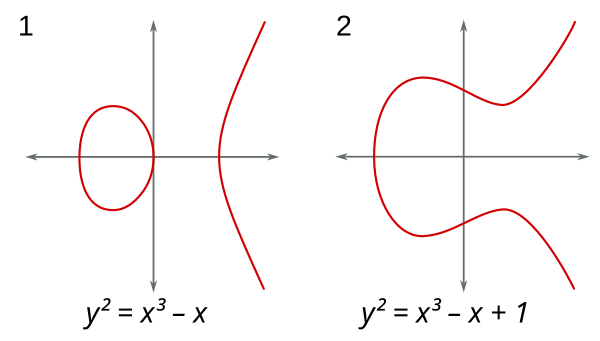
\includegraphics[width=0.5\linewidth]{img/curvas.png}
    \caption{Ejemplo de curvas elípticas}
    \label{fig:curvas}
\end{figure}

\subsection{Curvas elípticas sobre cuerpos finitos}

Nosotros no vamos a tratar sobre curvas continuas como son las que acabamos de ver sino con curvas definidas sobre cuerpos finitos, en concreto cuerpos del tipo $\mathbb F_{p^2}$. Estas curvas son visualmente bastante diferentes a las típicas gráficas a las que estamos acostumbrados, correspondiéndose más adecuadamente a una nube de puntos que a la línea continua que acabamos de ver.

\begin{figure}[h]
        \centering
    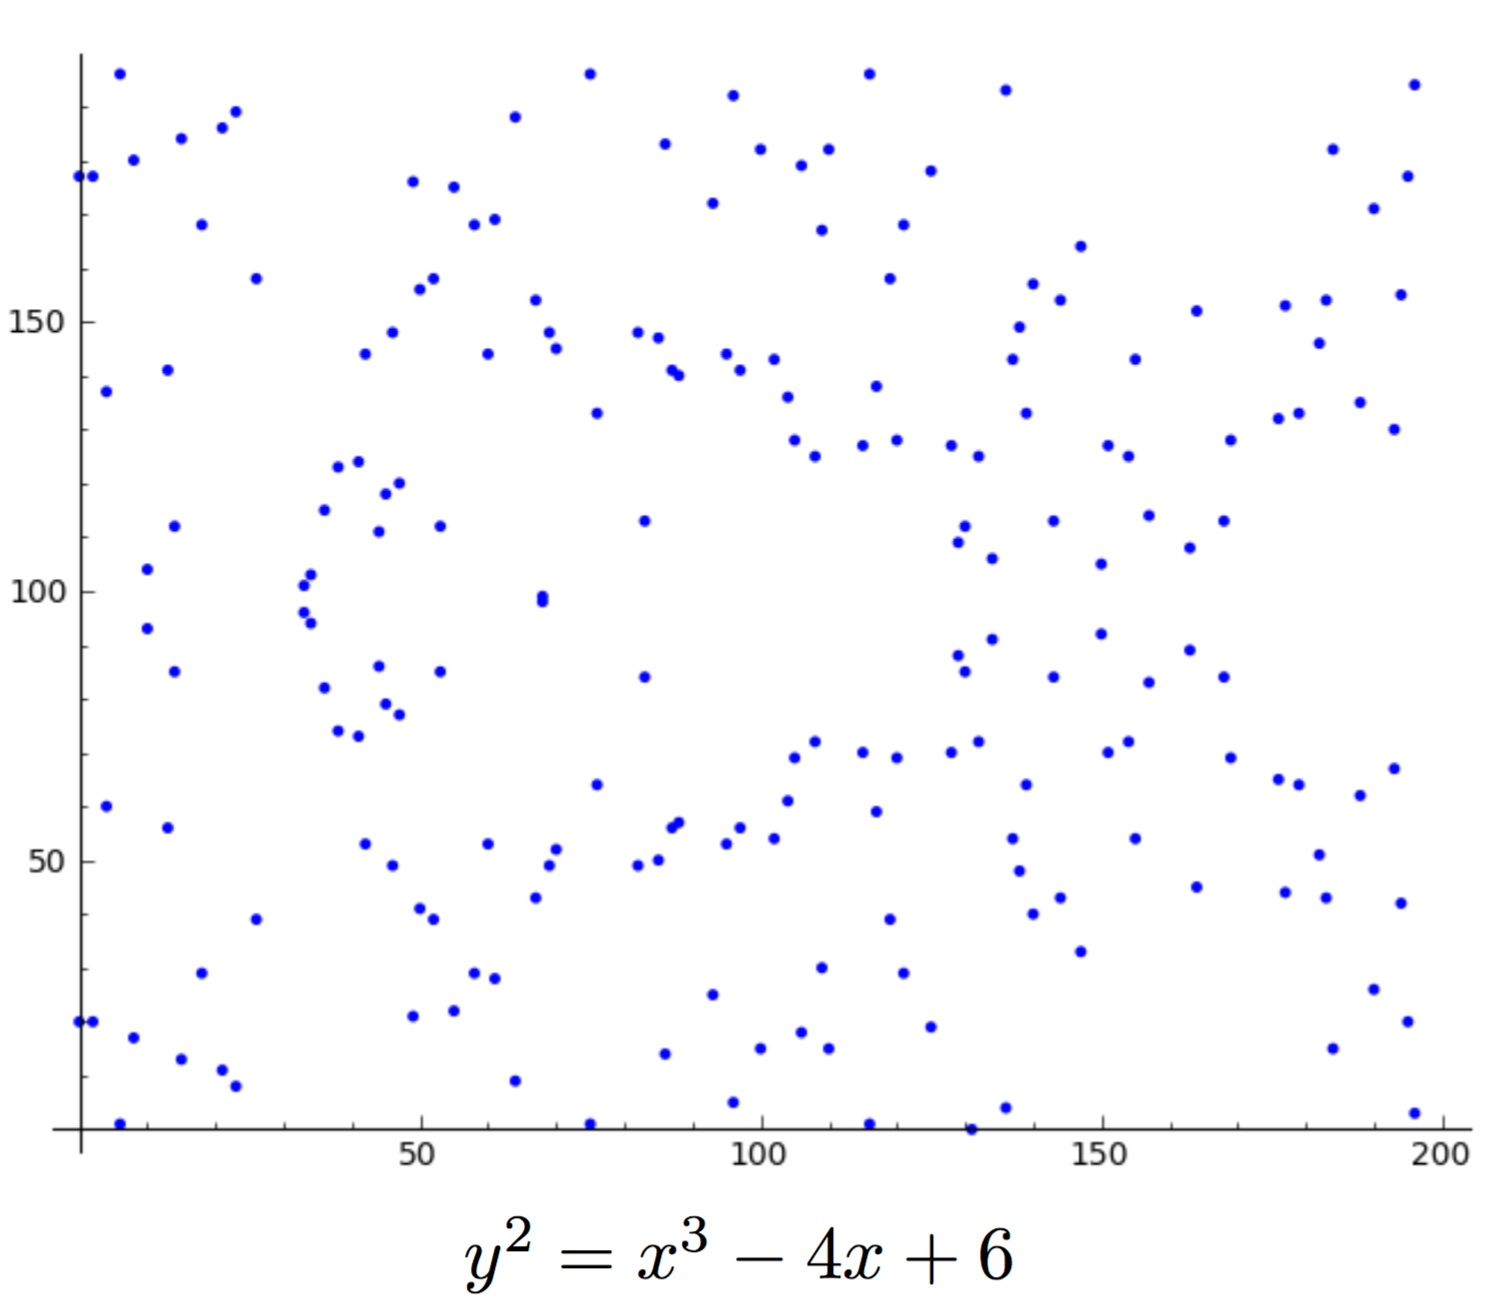
\includegraphics[width=0.7\linewidth]{img/curva-eliptica-finita.jpg}
    \caption{Curva elíptica definida sobre un cuerpo finito}
    \label{fig:curva-eliptica-finita}
\end{figure}

Sabiendo la composición de nuestro primo, que siempre va a ser de la forma $p=l_A^{e_A}l_B^{e_B}f \pm 1$ donde $l_A,l_B$ son primos pequeños\footnote{En concreto, estos primos pequeños serán $l_A=2,l_B=3$ ya que la diferencia en seguridad con primos más grandes no es tanta para la diferencia en velocidad que estos valores ofrecen.} sabemos que cualquier curva $E$ definida sobre el cuerpo $\mathbb F_{p^2}$ va a tener cardinalidad $(l_A^{e_A}l_B^{e_B}f)^2$.  A partir de aquí definimos el conjunto $E[l_A^{e_A}]$ que contiene a los $l_A^{e_A-1}(l_A+1)$ subgrupos cíclicos de orden $l_A^{e_A}$. Se construye el conjunto $E[l_B^{e_B}]$ de manera análoga.


\subsection{Curvas elípticas como grupos}

Como mencionamos en la sección anterior, los elementos de un conjunto pueden ser de la naturaleza que uno quiera. En este caso, vamos a tratar el conjunto de los puntos de una curva elíptica determinada.

Además de establecer este conjunto, las usaremos como grupo. Para ello, tenemos que definir previamente las operaciones que utilizaremos como operación de suma y multiplicación.

\subsubsection{Operación suma}

Dados dos puntos $P,Q \in E$, llamamos $L$ a la recta que une a estos dos puntos. Esta recta corta a la curva $E$ en un tercer punto $T$. Hacemos una segunda recta $L'$ que conecta el punto $T$ con el punto infinito $O$. $P+Q$ es, entonces, el tercer punto en el que la recta $L'$ intersecta a la curva $E$. En el caso de querer calcular el doble de un punto, la recta resultante será la tangente a la curva que pasa por ese punto. En las figuras \ref{fig:suma-distintos} y \ref{fig:suma-doble} incluimos ejemplos gráficos de la operación suma.

\begin{figure}[h]
    \centering
    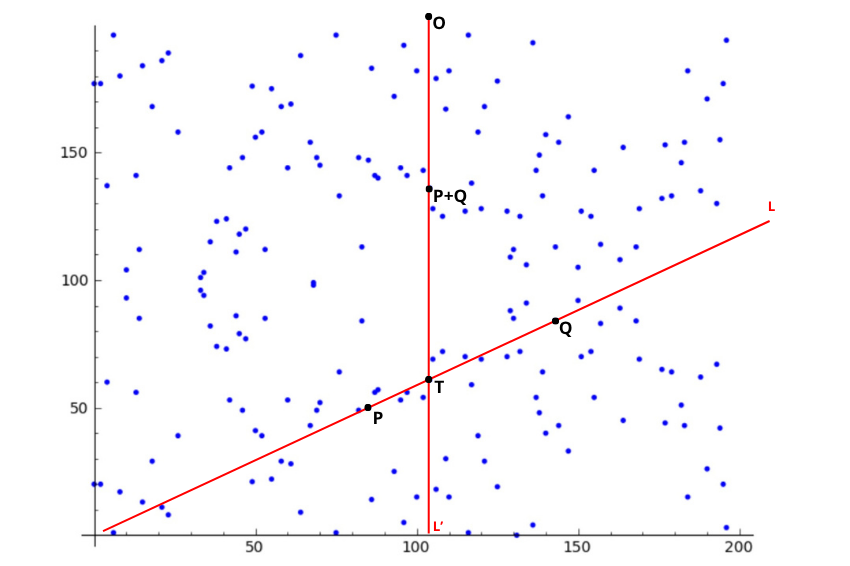
\includegraphics[width=0.7\linewidth]{img/suma.png}
    \caption{Operación suma para las curvas elípticas}
    \label{fig:suma-distintos}
\end{figure}


\subsection{Curvas elípticas supersingulares}

Tal y como dice el nombre del protocolo, SIKE no utiliza cualquier curva elíptica sino que se centra en aquellas denominadas supersingulares. Las curvas elípticas se dividen en las \textit{ordinarias} y las \textit{supersingulares}.

No vamos a entrar en mucho detalle en la definición de curva supersingular ya que implica un nivel de complejidad y formalidad demasiado alto. \footnote{Para profundizar en el tema, se puede consultar el artículo \textit{An Introduction to Supersingular Elliptic Curves  and Supersingular Primes} \cite{intro_supersingular_curves} o el capítulo V del libro \textit{The Arithmetic of Elliptic Curves} \cite{silverman-arithmetic}, base del artículo de Huynh.} A nivel general, una curva supersingular se diferencia de una ordinaria porque su anillo de endomorfismos es más grande de lo normal.

¿Por qué nos interesan entonces las curvas supersingulares y no las ordinarias? La respuesta es fácil: en la práctica, el caso supersingular ofrece un número de beneficios; instanciar construcciones eficientes es mucho más fácil, y los mejores ataques clásicos y cuánticos contra los problemas computacionales relacionados tienen complejidad exponencial. \cite{SIKE_beginners} Además, las curvas supersingulares funcionan como un cuerpo, es decir, que podemos tratar con ellas sin temor a toparnos, sin querer, con una ordinaria.

%
%   ISOGENIAS
%

\section{Isogenias}

Una isogenia es un tipo de morfismo con un kernel finito. De manera similar, una isogenia entre curvas elípticas es un morfismo de kernel finito entre dos curvas elípticas. Usando este concepto, podemos entender en qué consiste el protocolo. Una aplicación sigue siendo una aplicación aunque en vez de los número reales estemos tratando con curvas elípticas, y la base fundamental de nuestro protocolo va a ser la combinación de funciones.

\begin{figure}[!ht]
    \centering
    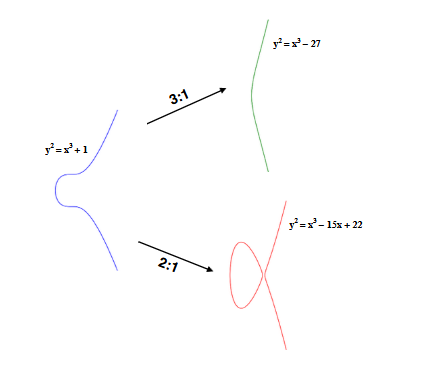
\includegraphics[width=0.5\linewidth]{img/isogeny-example.png}
    \caption{Ejemplo visual de isogenias}
    \label{fig:isogeny-example}
\end{figure}

\subsection{Isogenias duales}

Toda isogenia tiene lo que se denomina una isogenia dual. Estas isogenias se comportan, en mayor parte, como inversas. No técnicamente inversas ya que no son aplicaciones biyectivas, dos isogenias diferentes pueden tener una misma isogenia dual. Esto no tiene mucha repercusión a la hora de trabajar con ellas, ya que la isogenia dual existe y cumple sus propiedades. 

\subsection{Grado de una isogenia}

Al igual que una curva elíptica puede tomar múltiples formas, a la hora de definir una isogenia se puede hacer de miles de formas diferentes. La manera que vamos a tratar nosotros es mediante las fórmulas de Vélu \cite{velu}, que permiten, dada una curva Weierstrass $E$ de dominio y un conjunto finito de puntos $G$, definir una isogenia.

Este conjunto de puntos $G$ serán el kernel de la isogenia, esto es, los puntos cuya imagen será el origen, cuya dimensión definimos como el \textit{grado de la isogenia}. Además, cuando estamos hablando de una isogenia, podemos referirnos a ella como una $k$-isogenia, donde $k$ es su grado.

De esta forma, tenemos que conocer un subgrupo cíclico dentro de una curva dominio va a equivaler conocer una isogenia, su estructura y la curva imagen junto con su estructura de grupo. Las ecuaciones de Vélu nos permitirán pues calcular muy fácilmente todas las isogenias de un grado determinado a partir de una curva origen. Repitiendo el proceso conforme vamos encontrando curvas imagen, obtendremos de manera sencilla todas las isogenias definidas a partir de todas las curvas definidas sobre un mismo cuerpo.

%
%   INVARIANTES
%

\section{$j$-invariantes}

El $j$-invariante de una curva elíptica se puede calcular de varias maneras dependiendo de la forma que tome la curva.

\begin{description}
    \item[Forma de Weierstrass] Dada una curva de la forma $E: y^2 = x^3 + ax + b$, entonces su $j$-invariante se puede calcular mediante
    \[j(E) = 1728 \frac{4a^3}{4a^3 + 27b^2}\]

    \item[Forma de Montgomery] Dada una curva de la forma $E: y^2 = x^3 + ax^2 + x$, entonces su $j$-invariante se puede calcular mediante
    \[j(E) = 256 \frac{(a^2 - 3)^3}{a^2 - 4}\]
\end{description}

Aunque a primera vista uno pueda pensar que este valor va a ser único para cada curva, esto está lejos de la realidad. Por ejemplo, para $\mathbb{F}_{431^2}$ conseguimos un total de $37$ $j$-invariantes.

¿Para qué nos sirve esto? Los $j$-invariantes permiten agrupar las curvas elípticas de un cuerpo. Dos curvas con un mismo $j$-invariantes son isomórficas, lo que significa literalmente que tienen la misma forma. Es decir, desde un punto de vista matemático, dos curvas elípticas con un mismo $j$-invariante se podrían considerar la misma curva, no porque sus ecuaciones sean idénticas sino porque, al existir un isomorfismo entre ellas, sabemos que tienen las mismas propiedades.

Veamos una pequeña aclaración. Trabajando con las ecuaciones de Weierstrass, sean $E,E'$ dos curvas elípticas con el mismo $j$-invariante,

\[ E: y^2 = x^3 + Ax + B \]
\[ E' : y'^2 = x'^3 + A'x' + B' \]

Bajo la asunción que $j(E) = j(E')$ podemos hallar un isomorfismo de la forma $(x,y) = (u^2x', u^3y')$ donde, dependiendo de los valores de $A,B$ tenemos los siguientes valores de $u$

\begin{enumerate}
    \item \textit{Caso $A=0$ $(j=0)$: } $u=(B/B')^{1/6}$
    \item \textit{Caso $B=0$ $(j=1728)$: } $u=(A/A')^{1/4}$
    \item \textit{Caso $AB\neq0$ $(j\neq0)$: } $u=(A/A')^{1/4}=(B/B')^{1/6}$
\end{enumerate}

Mediante este isomorfismo, podremos trabajar con $E$ o $E'$ de forma casi indistinta. Para mayor nivel de detalle, consultar la proposición 1.4 del capítulo III, sección I de \textit{The Arithmetic of Elliptic Curves} de Silverman.

Claramente, a nivel matemático no es lo mismo que a nivel criptográfico. La pregunta entonces es, con lo que respecta a SIKE, ¿dos curvas con el mismo $j$-invariante son la misma? Pues depende del momento. Ya lo veremos con más detalle más adelante pero en un momento del intercambio de clave tenemos que calcular la imagen de unos puntos, por lo que ahí claramente no podemos considerar cualquier curva isomórfica como la misma, ya que nos interesa su valor concreto. Sin embargo, a la hora de encriptar un mensaje, utilizamos el $j$-invariante de la curva compartida el cual como acabamos de ver se mantiene entre isomorfismos.

Podríamos pensar que reducir tan drásticamente el número de valores es un contratiempo para nuestro protocolo, por el contrario, aunque el número de valores parece que desciende, las isogenias disponibles siguen siendo las mismas. Mediante nuestro protocolo nos interesa cambiar de $j$-invariante, más que de curva, ya que como acabamos de ver podríamos no haber hecho ninguna operación efectiva, matemáticamente.

%
%   GRAFOS DE ISOGENIAS
%

\section{Grafos de isogenias}

Una isogenia puede calcularse de mil maneras diferentes, la forma que utilizaremos define previamente el kernel de la isogenia y a partir de este y la curva dominio obtenemos la isogenia y la curva imagen. Siendo una isogenia cualquier morfismo 

\[\phi : E \to E'\]
\[\text{con }Ker(\phi) = K\] 

la curva imagen $E'$ suele ser definida como $E/K$, resultando en la siguiente ecuación

\[\phi : E \to E/K\]

que definiría exactamente la misma isogenia que la que hemos definido antes.

A partir de los $j$-invariantes, el orden de nuestro kernel y las fórmulas de Vélu \cite{velu}, tomando un primo $l$ diferente a nuestro primo $p$, podemos generar un grafo con las $l$-isogenias  entre los $j$-invariantes.

Este grafo tendría como nodos los $j$-invariantes y como aristas las mismas $l$-isogenias. Este grafo no sólo es útil computacional y matemáticamente sino que permitirá mostrar visualmente cómo funciona el protocolo de intercambio de claves de una forma muy intuitiva.

\subsection{Creación del grafo}

Veamos cómo creamos, paso a paso, un grafo de isogenias. Tomemos de punto de inicio el primo $p=431$, el cuerpo con el que vamos a trabajar entonces es $\mathbb F_{431^2}$.

Empezamos con una curva elíptica $E_0: y^2 = x^3 + (208i+161) x^2 + x$. Calculamos su $j$-invariante para una curva Montgomery y tenemos que 

\[j(E_0) = 256 \frac{((208i+161)^2 - 3)^3}{(208i+161)^2 - 4} = 364i+304 \]

Y de aquí obtenemos el primer nodo de nuestro grafo.

\begin{figure}[!ht]
    \centering
    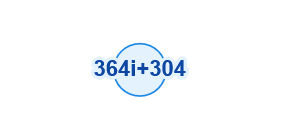
\includegraphics[width=0.33\linewidth]{img/isogeny-graph-step-1.png}
    \caption{Primer nodo del grafo}
    \label{fig:isogeny-graph-step-1}
\end{figure}

Una vez tenemos ya el primer nodo, vamos a seguir completando el grafo. A partir de nuestra curva $E_0$ vamos a tomar la $2$-isogenia

\[ \phi : E_0 \to E_1 \]
\[ \phi : x \mapsto \frac{x((350i + 68)x - 1}{x - (350i + 68)} \]

donde $E_1$ es la curva Montgomery $E_1 : y^2 = x^3 + (102i+423)x^2 + x$. Calculamos el $j$-invariante de $E_1$ y obtenemos que

\[j(E_0) = 256 \frac{((102i+423)^2 - 3)^3}{(102i+423)^2 - 4} = 344i+190 \]

Tenemos ya dos nodos y una arista en nuestro grafo.

\begin{figure}[!ht]
    \centering
    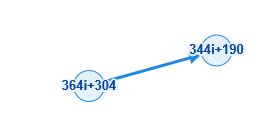
\includegraphics[width=0.5\linewidth]{img/isogeny-graph-step-2.png}
    \caption{Añadimos la primera arista al grafo}
    \label{fig:isogeny-graph-step-2}
\end{figure}

Sin embargo, a la hora de visualizar las aristas, aunque deberían ser dirigidas como lo acabamos de ver, vamos a tratar con un grafo no dirigido ya que, al existir las isogenias duales, se entiende que si existe una arista en una dirección, necesariamente existirá una en sentido contrario.

\newpage\begin{figure}[!ht]
    \centering
    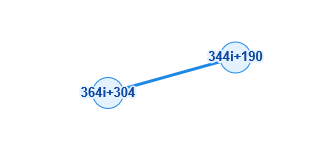
\includegraphics[width=0.5\linewidth]{img/isogeny-graph-step-3.png}
    \caption{Grafo no dirigido}
    \label{fig:isogeny-graph-step-3}
\end{figure}

Completando el grafo, llegaremos al siguiente grafo

\begin{figure}[!ht]
    \centering
    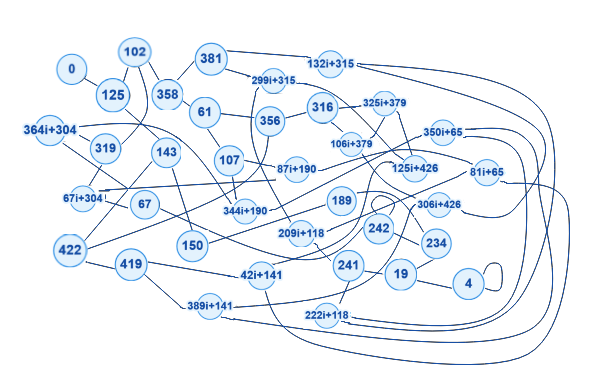
\includegraphics[width=1\linewidth]{img/isogeny-graph.png}
    \caption{Grafo de $2$-isogenias para $p=431$}
    \label{fig:isogeny-graph}
\end{figure}

     \chapter{Estudio teórico de las bases del protocolo}\label{estudioteorico}

%
% PROBLEMA CUANTICO
%

\section{La computación cuántica y sus consecuencias en criptografía }

La criptografía es la base de nuestros sistemas informáticos ya que nos proporciona la seguridad necesaria para comunicarnos y tratar con cualquier tipo de información, de la más sensible a la menos. Las consecuencias de que no podamos confiar en esta seguridad sobre la que dependemos serían catastróficas, y justo eso es lo que amenaza hacer los ordenadores cuánticos.

Los ordenadores cuánticos no son sólo una amenaza por su velocidad y sus recursos propios sino que en 1994, Peter Shor publicó lo que hoy en día se conoce cómo algoritmo de Shor, posiblemente el más famoso de los algoritmos cuánticos a día de hoy. Este algoritmo permitiría resolver los problemas del logaritmo discreto y de la factorización de un número en tiempo polimonial. Estos problemas son la base de la mayoría de los protocolos criptográficos que utilizamos hoy en día por lo que una implementación en un ordenador cuántico de este algoritmo podría rebasar cualquier sistema de seguridad actual.

Uno de estos algoritmos en peligro es Diffie-Hellman, la base de la criptografía de clave pública. La seguridad de este protocolo reposa en la complejidad computacional del Problema Computacional Diffie-Hellman (CDHP por sus siglas en inglés) que trata lo que es conocido como el problema del logaritmo discreto (DLP).

\begin{problem}[Problema del logaritmo discreto]
    Dado $\alpha \in G$ y $\beta \in \langle \alpha \rangle$ encontrar el menor entero $x$ tal que $\alpha^x = \beta$. \cite{discrete-logarithm}
\end{problem}

Este problema ha sido adaptado de muchas formas, entre otras, a curvas elípticas. Esta adaptación toma la estructura de grupo de las curvas elípticas con la multiplicación escalar y aplica el concepto del logaritmo discreto, lo que se convierte en el ECDLP o Problema del Logaritmo Discreto en Curvas Elípticas.

Los algoritmos de Shor permitirían romper el problema del logaritmo discreto en tiempo polinomial en contraste con la complejidad exponencial de un algoritmo clásico,\footnote{Realmente, los algoritmos de Shor no son deterministas sino probabilísticos, es decir, no dan siempre el resultado correcto sino que lo encuentran un gran número de veces. No obstante, esto es suficiente para poner en peligro nuestra seguridad actual.} y aunque no se considera probable que se vayan a desarrollar ordenadores cuánticos que puedan implementar estos algoritmos en los próximos años (en la figura \ref{fig:expert-estimates} mostramos un gráfico proporcionado por el Global Risk Institute \cite{quantum-threat-timeline}), el proceso de migración utilizando los recursos que ahora mismo tenemos disponibles se estima que pueda tomar más de cinco años tomando de referencia transiciones previas \cite{coordinated-implementation-roadmap}.

\begin{figure}[!ht]
    \centering
    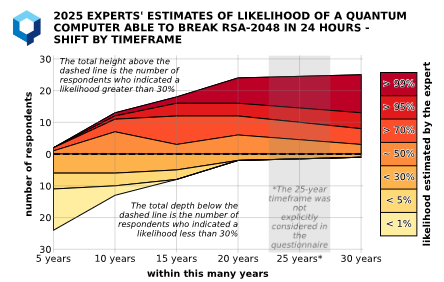
\includegraphics[width=0.75\linewidth]{img/expert-estimates.png}
    \caption{Un gráfico de área apilado que refleja los datos obtenidos, ofreciendo una visión clara de cómo las estimaciones cambian del corto al largo plazo: por cada rango horario, la altura total de la línea rayada indica el número de encuestados que estiman al menos una probabilidad del 30 por ciento.}
    \label{fig:expert-estimates}
\end{figure}

El National Institute of Standards and Technology o NIST, un organismo estadounidense perteneciente al ministerio de comercio que, entre otros objetivos, busca establecer unos estándares de seguridad capaces de hacer frente a la capacidad de los ordenadores cuánticos.

Esto es lo que se conoce como criptografía post-cuántica, no porque utilice algoritmos ni ordenadores cuánticos sino porque es resistenete a estos. Estos protocolos se basan en problemas matemáticos que deben ser resistentes tanto a ataques clásicos como a ataques cuánticos.

A lo largo de 2016 el NIST hizo una llamada general, presentó el concepto de criptografía post-cuántica y propuso unos plazos para encontrar candidatos a estandarización. La primera de las cuatro rondas se abrió en diciembre de ese año, cerrándose casi un año más tarde, en noviembre del 2017.

A finales de este año se presentaron los algoritmos que habían superado los requisitos mínimo de esta ronda, un total de 69. La segunda ronda se cerró en enero de 2019 y estuvo compuesta de 26 candidatos mientras que la tercera, en julio de 2020, se compuso de 15, 8 nominados y 7 alternos. La cuarta y última ronda se cerró en 2022, proponiendo los candidatos a estandarización \cite{nist-timeline}.


%
% SIDH vs SIKE
%

\section{SIDH vs SIKE}

SIKE (Super-singular Isogeny Key Encapsulation) \cite{sike-org}  \cite{SIKE} se postula como una adaptación de Diffie-Hellman con isogenias de curvas elípticas. Sin embargo, es posible que hayas oído hablar de otro protocolo que se llama, literalmente, Super-singular Isogeny Diffie-Hellman o SIDH. La duda que muchos se harán al encontrarse con estos dos conceptos es, razonablemente, cual es la diferencia entre uno y otro.

La respuesta es fácil, SIKE es una variación de SIDH. SIDH permite una mayor variabilidad al contar con un juego de parámetros libres, en concreto, el tamaño del primo. SIKE es, específicamente, la versión concreta presentada a las convocatorias del NIST. En ella, los autores definen cuatro posibles sets de parámetros: SIKEp434, SIKEp503, SIKEp610, SIKEp751 \cite{SIKE_specifications}.

\begin{table}[h]
    \centering
    \begin{tabular}{|p{0.17\linewidth}||p{0.17\linewidth}|p{0.16\linewidth}|p{0.16\linewidth}|p{0.16\linewidth}|}
         \hline
        Parámetros & Nivel de seguridad según el NIST & Clave privada (bytes) & Clave pública (bytes) & Secreto compartido (bytes)\\ \hline
        SIKEp434 & 1 & 374 & 330 & 16\\ \hline
        SIKEp503 & 2 & 424 & 378 & 24\\ \hline
        SIKEp610 & 3 & 524 & 462 & 24\\ \hline
        SIKEp751 & 5 & 644 & 564 & 32\\ \hline
    \end{tabular}
    \caption{Sets de parámetros proporcionados por SIKE}
    \label{tab:sike_parameters}
\end{table}

%
% FUNCIONAMIENTO DEL PROTOCOLO
%

\section{Funcionamiento del protocolo}

 \subsection{Resumen en lenguaje cercano}

 El protocolo presentado por de Feo, Jao y Plût utiliza el esquema clásico de Diffie-Hellman, la diferencia principal se encuentra en el contenido de la clave, en qué problema matemático se utiliza por detrás de estos esquemas ya probados para añadirle la seguridad que le falta a la criptografía clásica.
 
En vez del problema del logaritmo discreto como base de la seguridad y complejidad de SIKE, los autores han apostado por la composición de funciones, en concreto, de isogenias supersingulares.

Para conseguir el secreto conjunto, los usuarios parten de una curva pública común. Cada uno por separado, le aplican a esta misma curva una serie de transformaciones llegando a unas curvas intermedias independientes. Llegados este punto, intercambian las imágenes de estos puntos públicos originales que utilizarán para continuar las transformaciones. De esta forma consiguen llegar a un secreto común sin haber compartido las isogenias que han utilizado.

En un primer momento, se consideró que estos puntos intermedios que se comparten en claro no suponían un peligro para el secreto, por ello el protocolo pasó hasta la tercera ronda del NIST. Sin embargo, en Julio de 2022, Wouter Castryck y Thomas Decru publicaron un ataque efectivo contra el protocolo utilizando estos puntos \cite{efficient_attack}.

\begin{comment}
%
% PRUEBA DE IDENTIDAD
%

\subsection{Prueba de identidad}

El protocolo de identidad ideado por De Feo, Jao y Plût se basa en el siguiente esquema:

\begin{figure}[!ht]
    \centering
    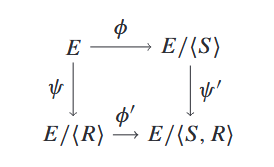
\includegraphics[width=0.3\linewidth]{img/Zero-knowledge graph.png}
    \caption{Diagrama sobre el que reposa la idea de la prueba de identidad}
    \label{fig:proof_of_identity}
\end{figure}

donde $\langle S \rangle$ es el kernel de la isogenia secreta $\phi$ de grado $l_A^{e_A}$ y $\langle R \rangle$ es un grupo cíclico de orden $l_B^{e_B}$. Los usuarios, utilizaremos Alice y Bob, pueden computarlo fácilmente utilizando las fórmulas de Vélu y calculando las isogenias a partir de las imágenes de los puntos.

El problema es entonces qué puede Alice desvelar del diagrama para demonstrar su identidad sin comprometer su secreto $\phi$. No puede ser $(\psi, \phi’)$ ó $(\psi’, \phi’)$ ya que estos permiten fácilmente computar $Ker(\phi)$. Finalmente, nos decantamos por $(\psi, \psi’)$.

\subsubsection{Parámetros públicos y secretos}

\begin{description}
    \item Parámetros públicos
        \begin{enumerate}
            \item Curvas elípticas supersingulares $E, E/\langle S \rangle$.
            \item Generadores $P,Q$ de $E[l_B^{e_B}]$ y sus imágenes $\phi(P),\phi(Q)$.
        \end{enumerate}
    \item Parámetros secretos
        \begin{enumerate}
            \item Punto de $l_A^{e_A}$-torsión $S$ que define
            \item La isogenia $\phi : E \to E/\langle S \rangle$.
        \end{enumerate}
\end{description}

\subsubsection{Pasos del protocolo}

Los siguientes pasos se repetirán un número $m$ de veces.

\begin{enumerate}
    \item Alice escoge un punto aleatorio $l_B^{e_B}$-torsión $R$ y computa el diagrama anterior.
    \item Alice le envía a Bob las curvas $E / \langle R \rangle, E/ \langle S,R \rangle$.
    \item Bob escoge un bit aleatorio $b$ y se lo envía a Alice.
        \begin{itemize}
            \item Si $b = 0$, Alice revela $R, \phi(R')$ y, si tienen orden $l_B^{e_B}$, Bob genera los kernel de las isogenias $E \to E / \langle R \rangle, E/\langle S \rangle \to E/ \langle S,R \rangle$, respectivamente.
            \item Si $b=1$, Alice revela $\psi(S)$ y, si tiene orden $l_A^{e_A}$, Bob genera el kernel de la isogenia $E / \langle R \rangle \to E/ \langle S,R \rangle$.
        \end{itemize}
\end{enumerate}
\end{comment}

%
% INTERCAMBIO DE CLAVES
%

\subsection{Intercambio de claves}

El intercambio de claves que propone SIKE es una adaptación de Diffie-Hellman en el que los usuarios computan isogenias individuales y a partir de estas crean la clave compartida.

\subsubsection{Parámetros}

Empezamos definiendo los siguientes parámetros públicos compartidos:

\begin{enumerate}
    \item Un primo $p=l_A^{e_A} \cdot l_B^{e_B} \cdot f \pm 1$.
    \item Una curva elíptica $E_0$ definida sobre $\mathbb{F}_{p^2}$.
    \item Un par de puntos $\{ P_A,Q_A \}, \{ P_B,Q_B \}$ para Alice y Bob respectivamente donde $\langle P_A,Q_A \rangle = E[l_A^{e_A}]$ , análogamente con $\langle P_B, Q_B \rangle$.
\end{enumerate}

\subsubsection{Pasos del protocolo}

Una vez establecemos estos valores, comienza el proceso de intercambio de clave. Trataremos sólo los pasos de Alice por simplificar la explicación, ya que Bob sigue el mismo proceso, aunque los valores específicos cambien.

Alice escoge un par de valores cualesquiera $m_A,n_A$ pertenecientes al grupo $\mathbb{Z}/ l_A^{e_A} \mathbb{Z}$, con ambos no divisibles por $l_A$. A partir de estos dos valores computa una primera isogenia $\phi_A$ con

\[Ker(\phi_A) = K_A := \langle [m_A]P_A + [n_A]Q_A \rangle\]

Una vez tiene definida este morfismo, computa las imágenes de los puntos base de Bob, es decir, $\phi_A(P_B), \phi_A(Q_B)$. En este punto del proceso, Alice y Bob intercambian la siguiente tupla de información $(E_A, \{ \phi_A(P_B), \phi_A(Q_B) \})$ y recibe una equivalente de parte de Bob. A partir de estos puntos intermedios, Alice calculará una nueva isogenia $\phi_A’$ con

 \[Ker(\phi_A) = K_A := \langle [m_A]\phi_B(P_A) + [n_A]\phi_b(Q_A) \rangle\]
 
De esta forma consiguen llegar a un $j$-invariante común que usarán de clave compartida.

 \[E_{AB} = \phi_B’(\phi_A(E_0)) = \phi_A’(\phi_B(E_0)) \rangle\]

Para simplificar la comprensión del protocolo, incluimos el esquema en la figura \ref{fig:diagrama}.

\newpage
\begin{figure}[!h]
    \centering
    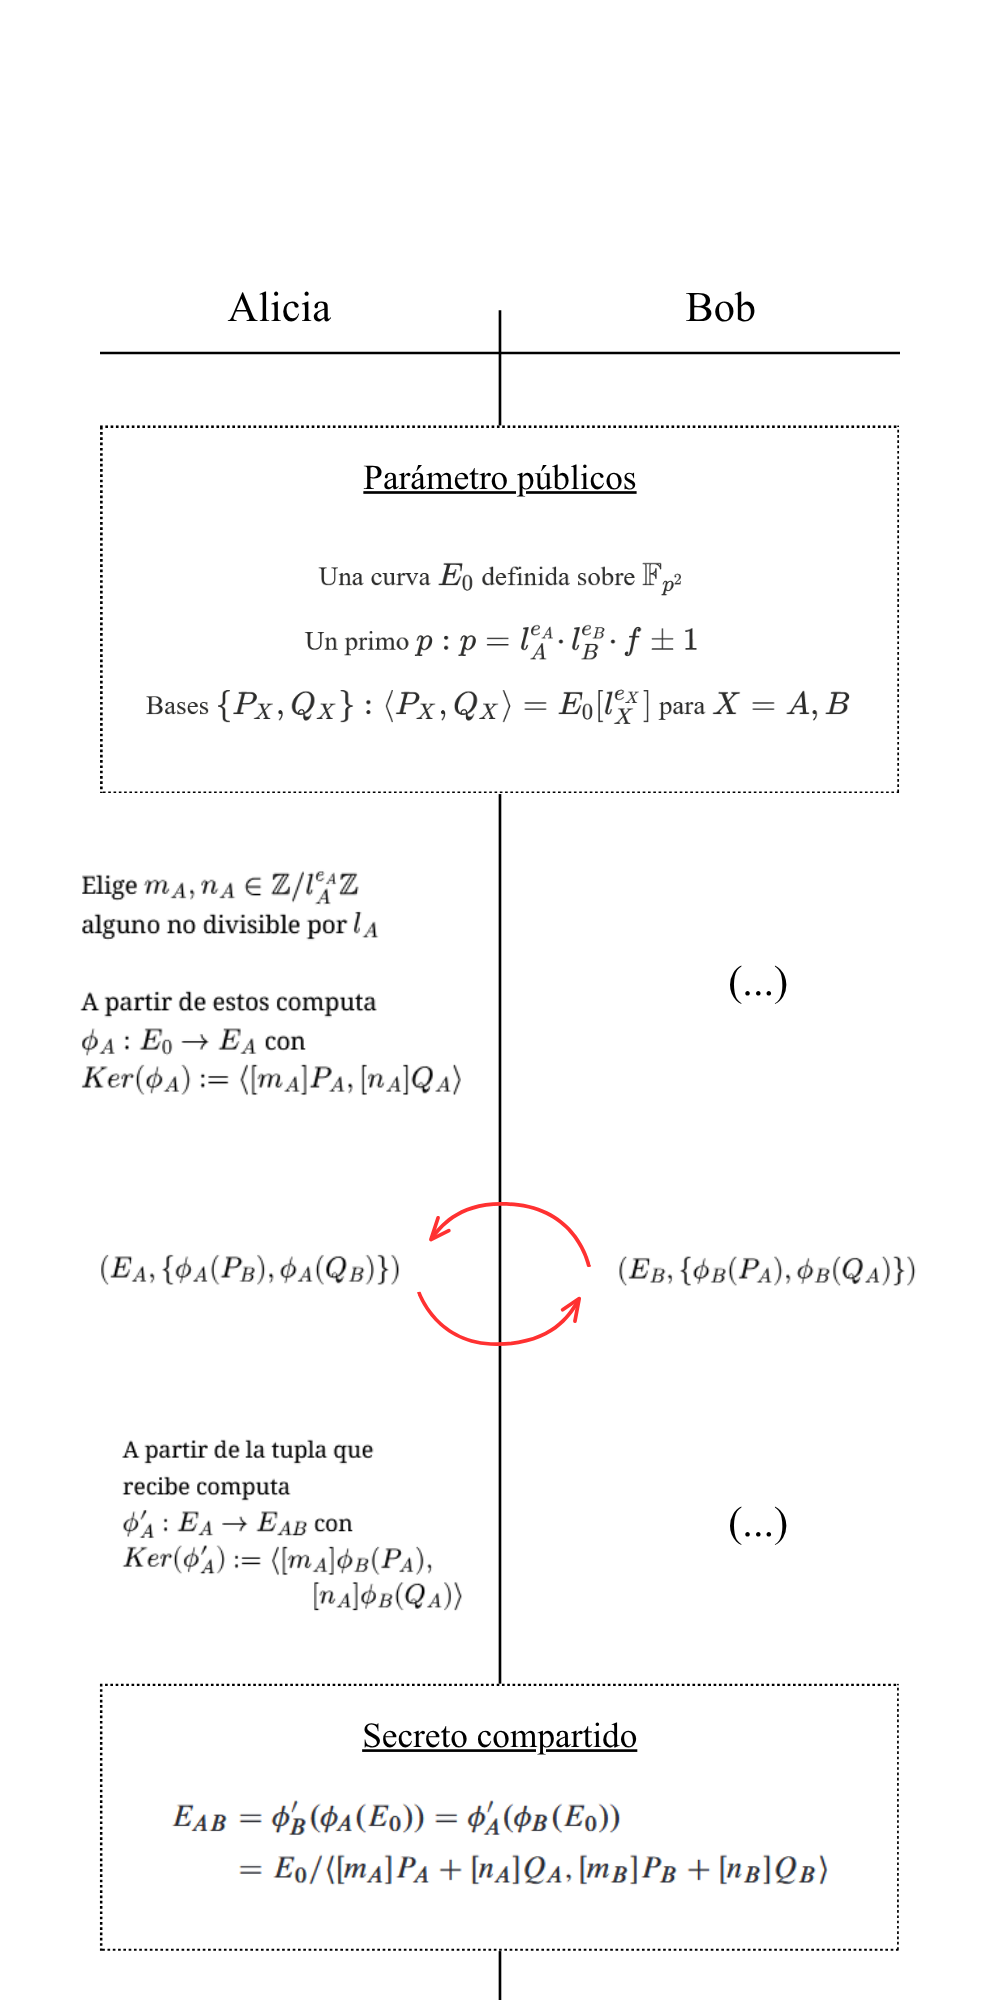
\includegraphics[width=0.75\linewidth]{img/Key exchange.png}
    \caption{Diagrama explicativo del protocolo de intercambio de clave}
    \label{fig:diagrama}
\end{figure}

\newpage
\subsubsection{Visualización del protocolo}

Comprender cómo funciona el intercambio de claves resulta mucho más sencillo si vemos el viaje que Alice y Bob realizan a través de un grafo de isogenias concreto. Pongamos de ejemplo el primo $p = 433$. En la figura \ref{fig:grafos-base} encontramos los grafos 2 y 3 isogenias de este primo por los datos proporcionados por la base de datos \textit{Isogeny graphs of supersingular elliptic curves} \cite{isogeny-graphs-ddbb}.

\begin{figure}[!h]
\begin{subfigure}[h]{0.4\linewidth}
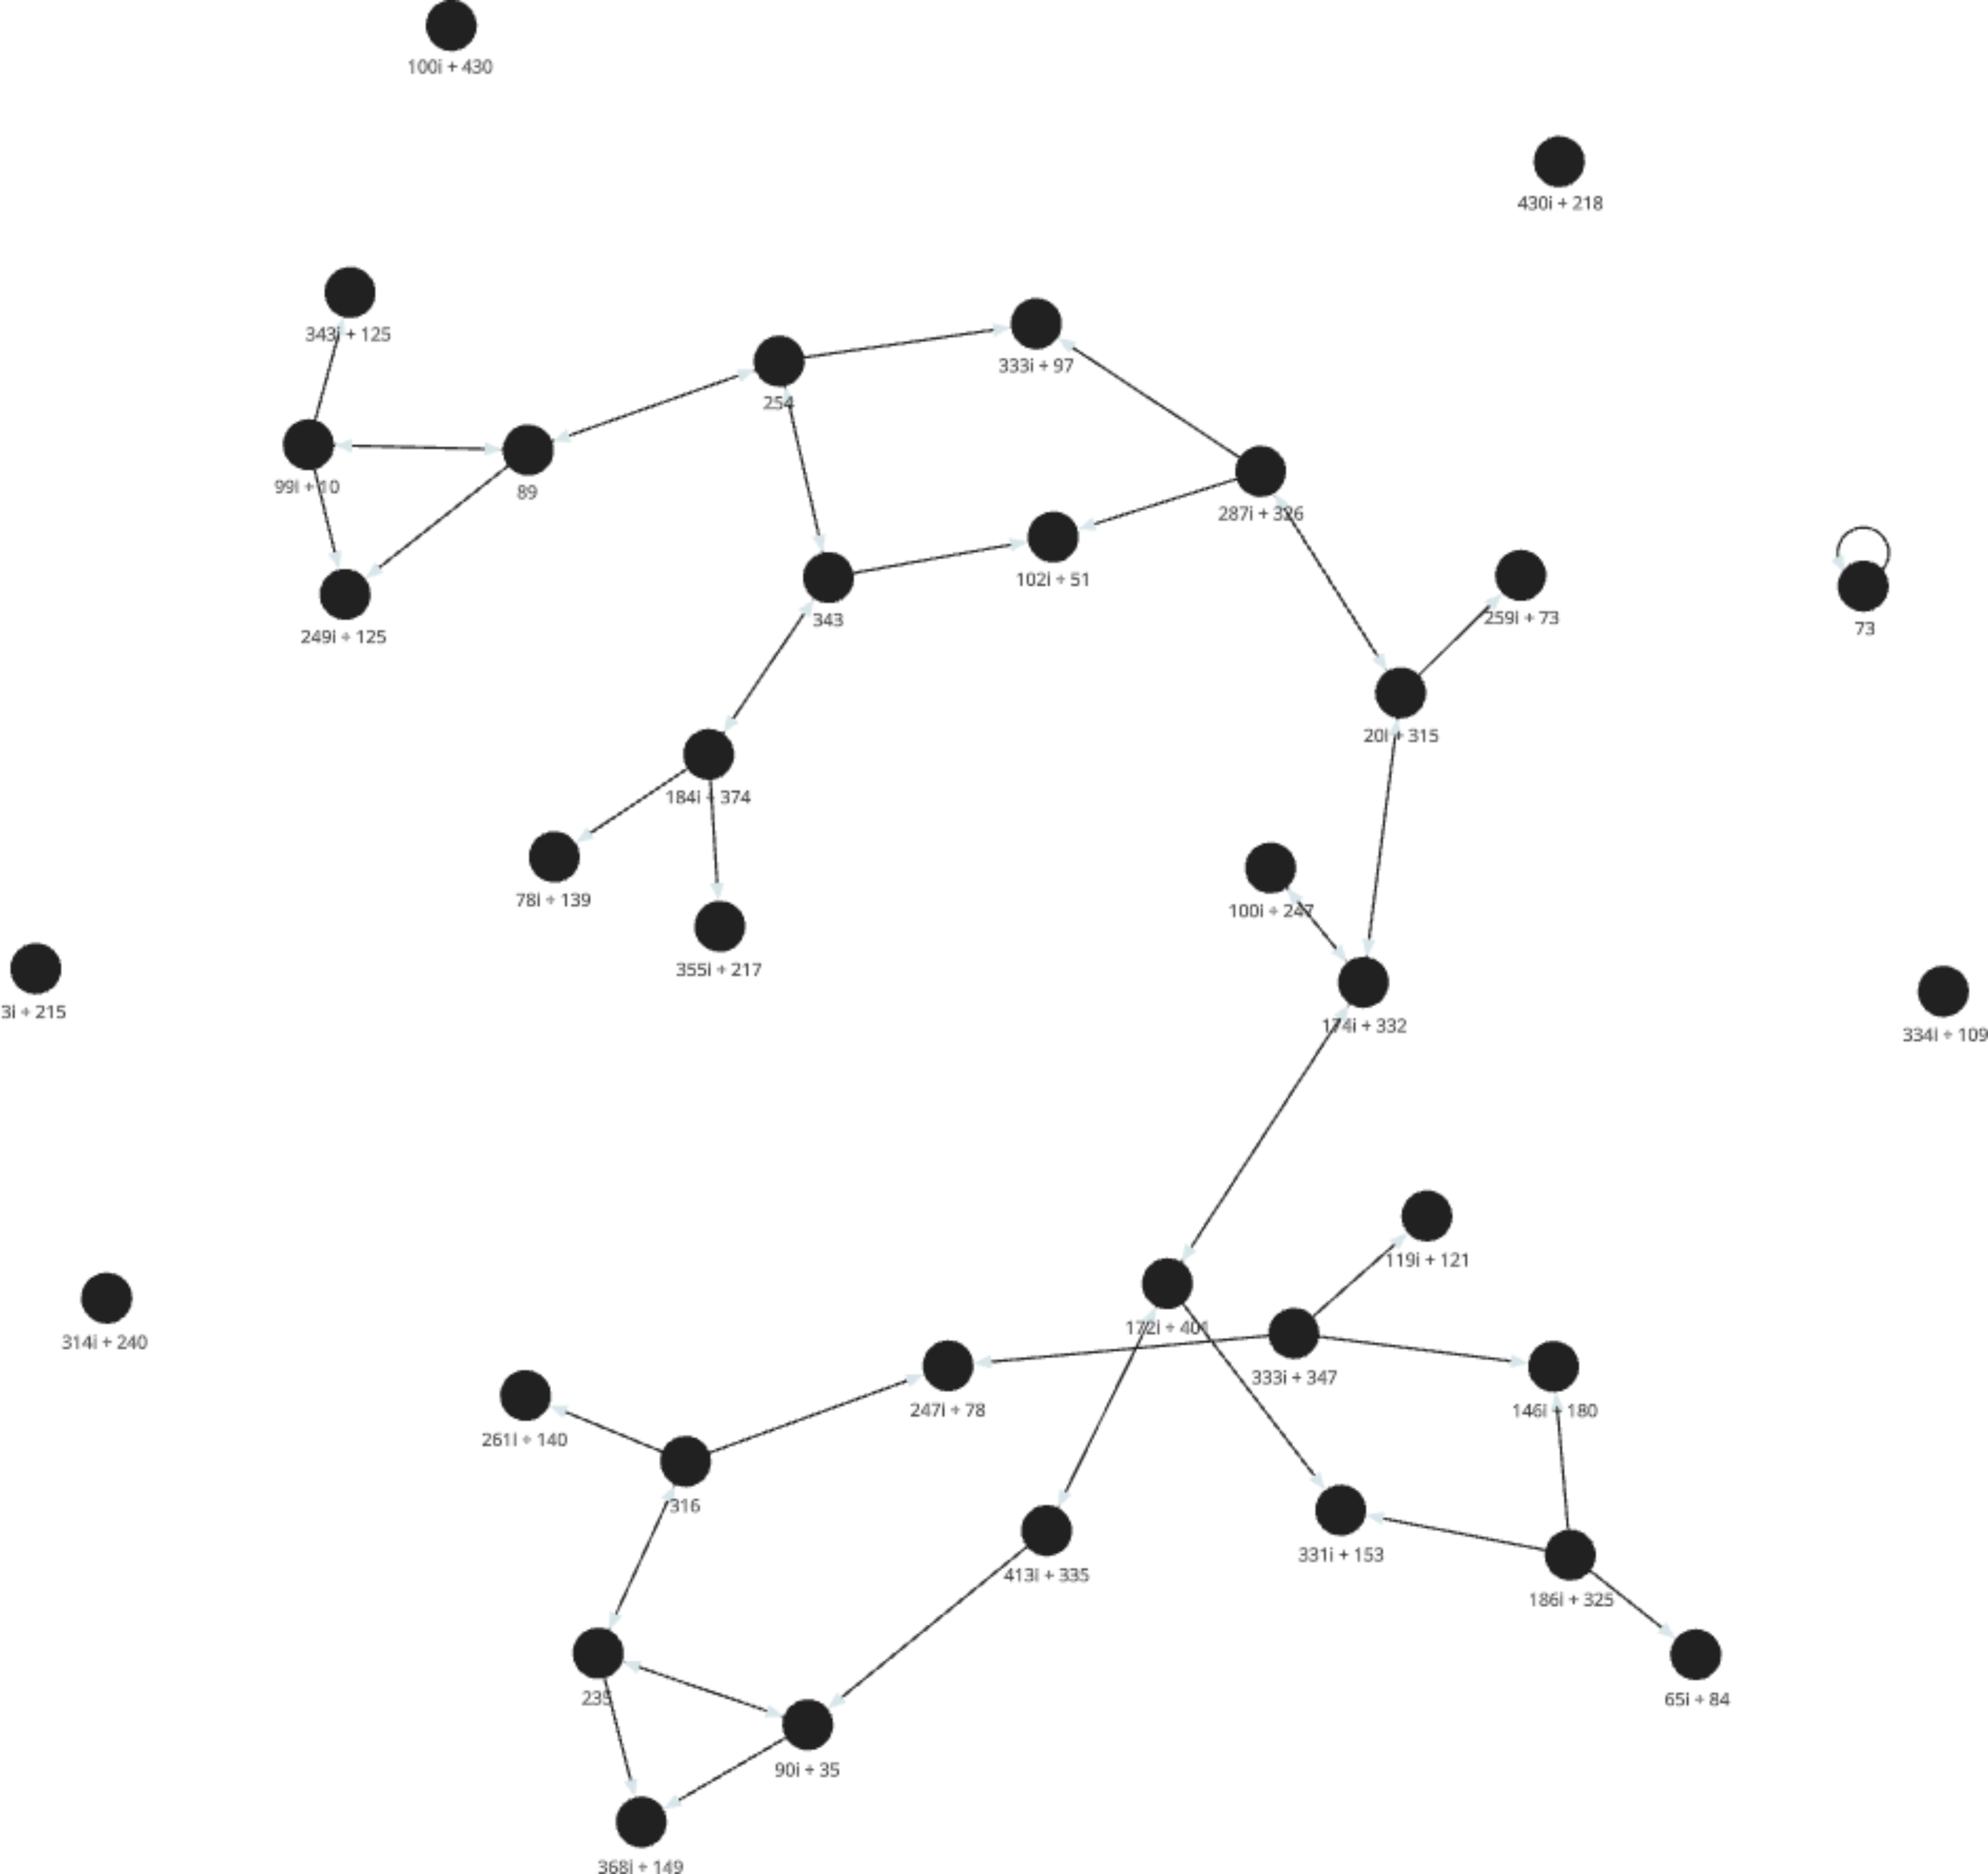
\includegraphics[width=\linewidth]{img/2-isogeny/2-isogeny.png}
\caption{Grafo de 2-isogenias}
\end{subfigure}
\hfill
\begin{subfigure}[h]{0.4\linewidth}
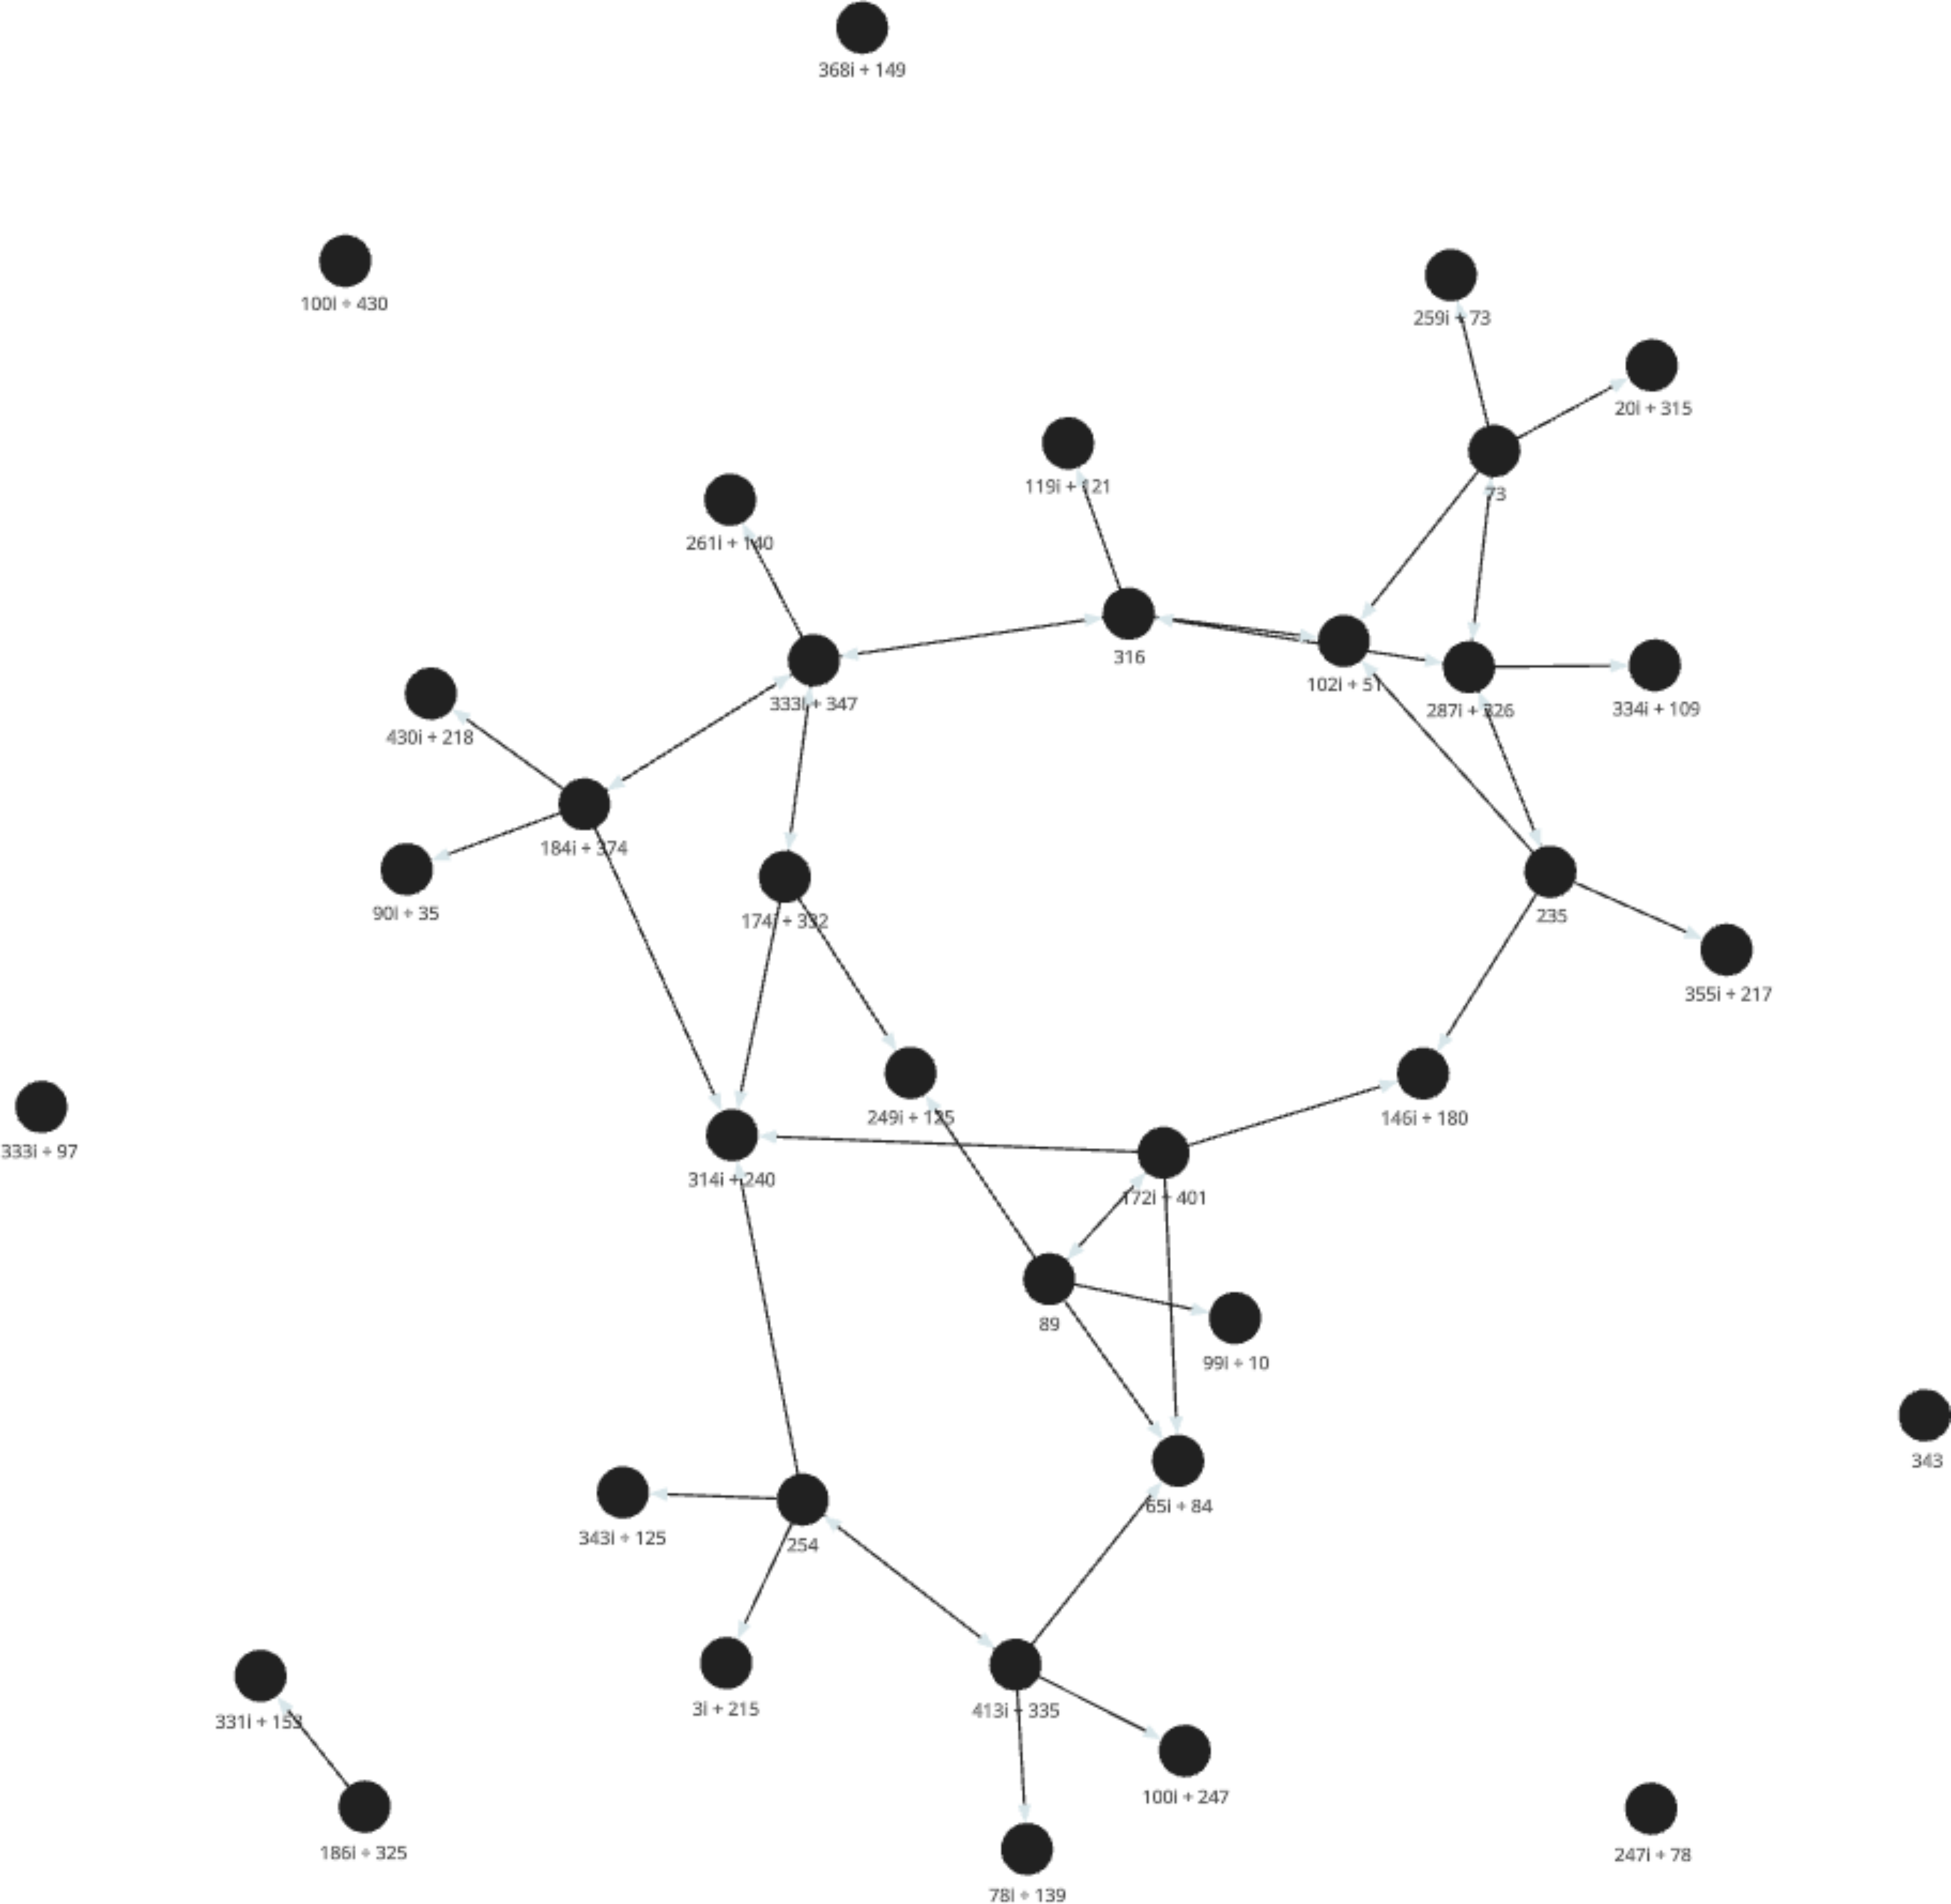
\includegraphics[width=\linewidth]{img/3-isogeny/3-isogeny.png}
\caption{Grafo de 3-isogenias}
\end{subfigure}
\caption{Grafos de isogenias para $p=433$}
\label{fig:grafos-base}
\end{figure}

Al calcular las isogenias intermedias propias de Alice y Bob, estos se desplazan por el grafo de isogenias. La factorización del primo escogido tiene gran importancia en este punto, ya que va a definir cómo estos se mueven por el grafo. Hemos escogido el primo $433$ que se puede factorizar de la siguiente forma $p = 433 = 2^4 \cdot 3^3 + 1$. Tenemos entonces que $l_A = 2, e_A = 4$ y $l_B = 3, e_B = 3$\footnote{Puede ser al revés, pero en este ejemplo trataremos con estos valores.}. Alice entonces, se desplazará a través de 4 nodos en el grafo de 2-isogenias mientras que Bob atravesará 3 nodos en el de 3-isogenias. En la figura \ref{fig:grafos-intermedio} encontramos un ejemplo de esta primera parte del camino.

\begin{figure}[!h]
\begin{subfigure}[h]{0.4\linewidth}
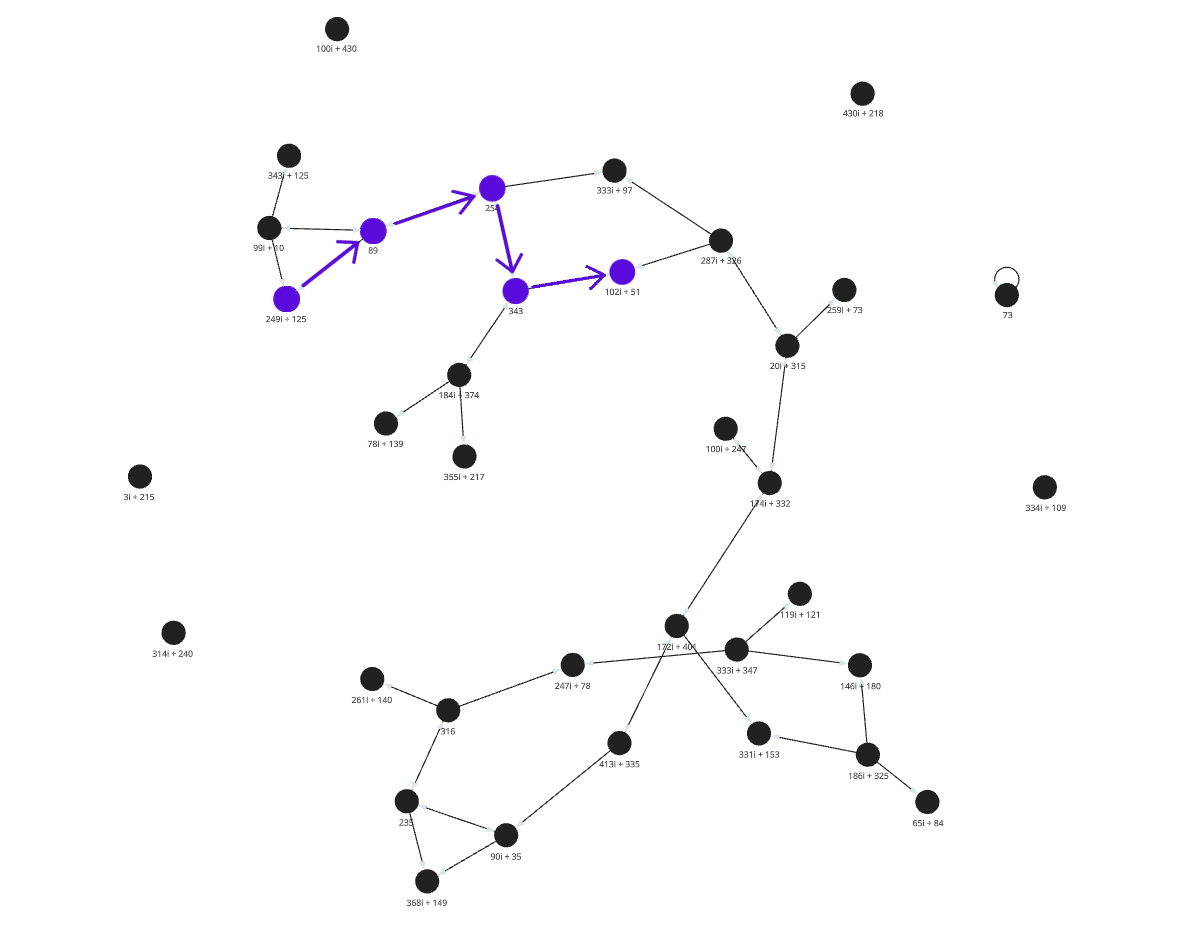
\includegraphics[width=\linewidth]{img/2-isogeny/step4.png}
\caption{Camino por el grafo de 2-isogenias}
\end{subfigure}
\hfill
\begin{subfigure}[h]{0.4\linewidth}
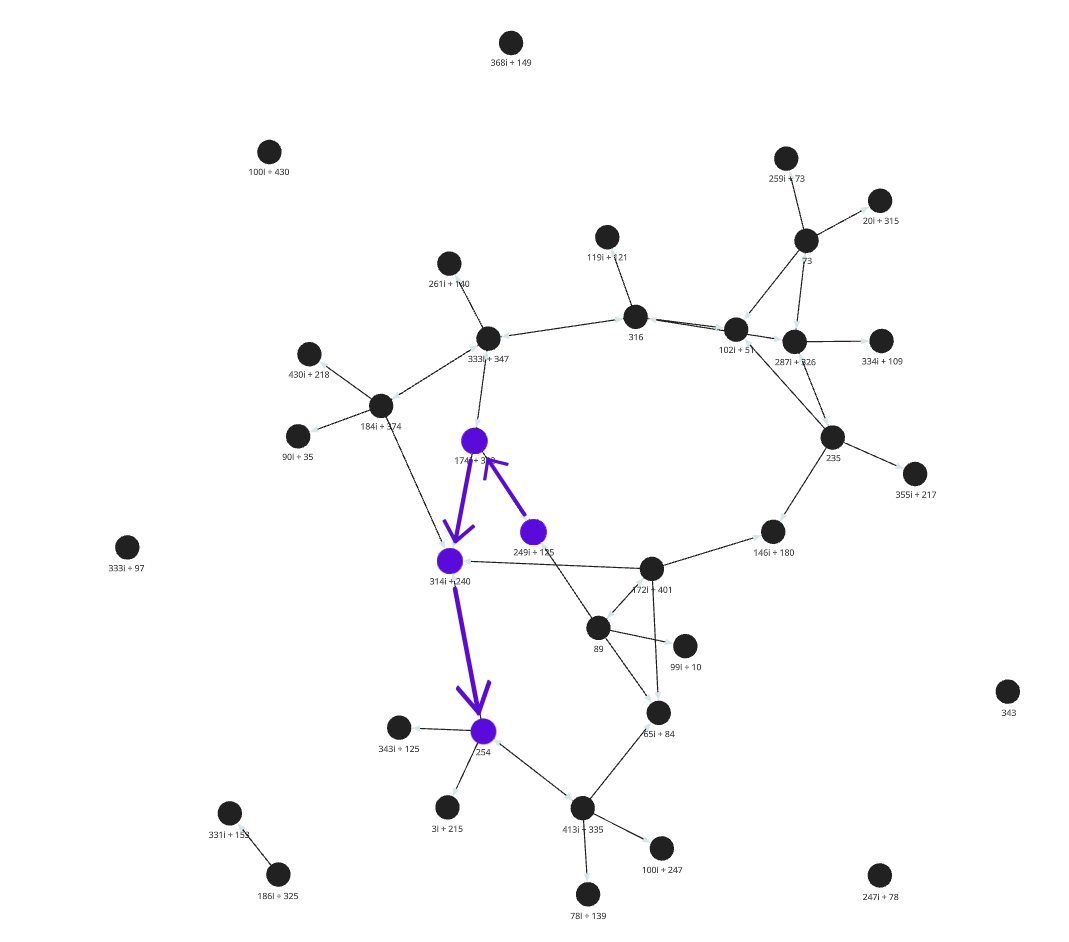
\includegraphics[width=\linewidth]{img/3-isogeny/step3.png}
\caption{Camino por el grafo de 3-isogenias}
\end{subfigure}
\caption{Caminos por los grafos de isogenias para $p=433$}
\label{fig:grafos-intermedio}
\end{figure}

Es en este punto en el que Alice y Bob calculan las imágenes de los puntos iniciales del otro y se las intercambian. Una vez tienen estos puntos intermedios, vuelven a desplazarse a través del grafo para llegar a una misma curva $E_{AB}$. En la figura \ref{fig:grafos-final} mostramos esta segunda parte del viaje mientras que en la \ref{fig:grafos-invariante} mostramos en concreto el nodo final del desplazamiento.

\begin{figure}[!h]
\begin{subfigure}[h]{0.4\linewidth}
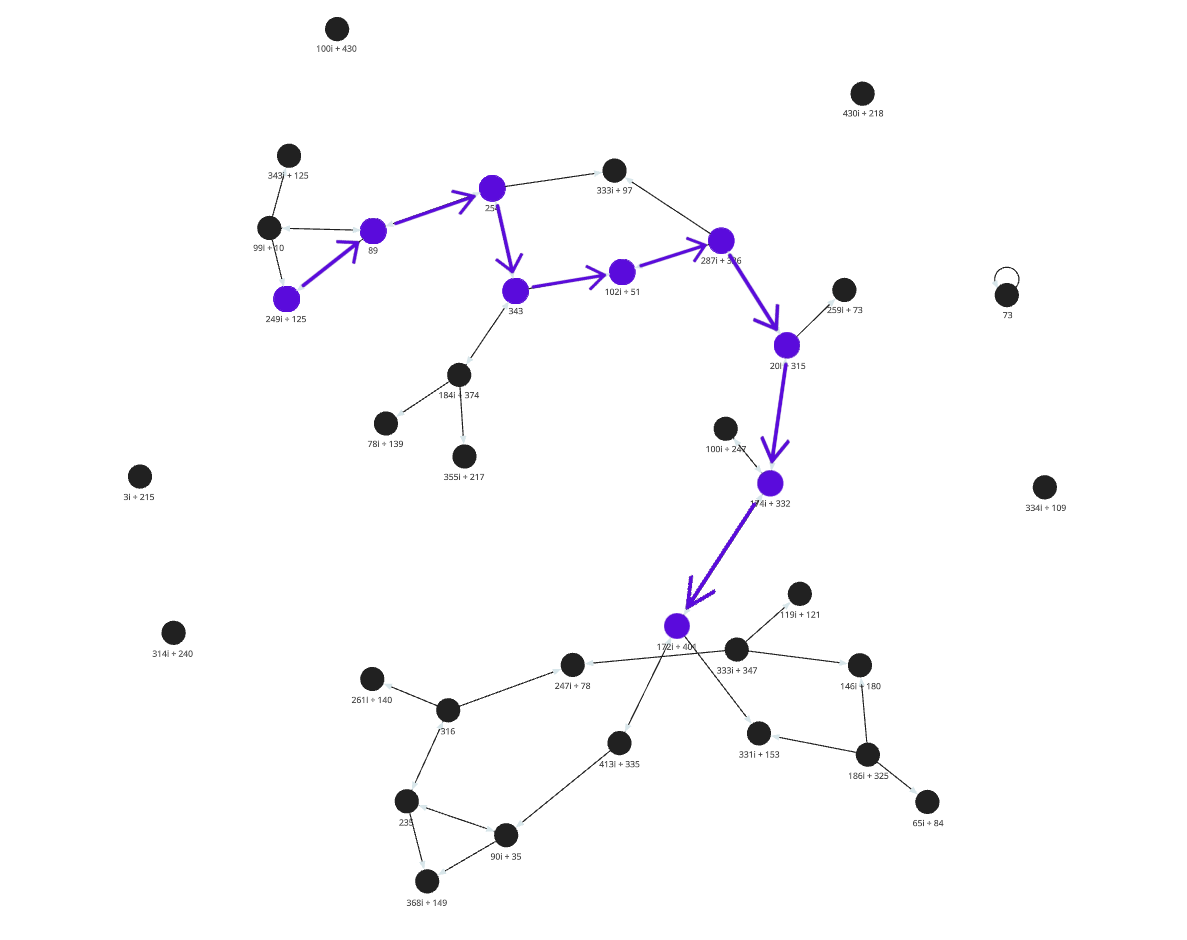
\includegraphics[width=\linewidth]{img/2-isogeny/step8.png}
\caption{Camino final por el grafo de 2-isogenias}
\end{subfigure}
\hfill
\begin{subfigure}[h]{0.4\linewidth}
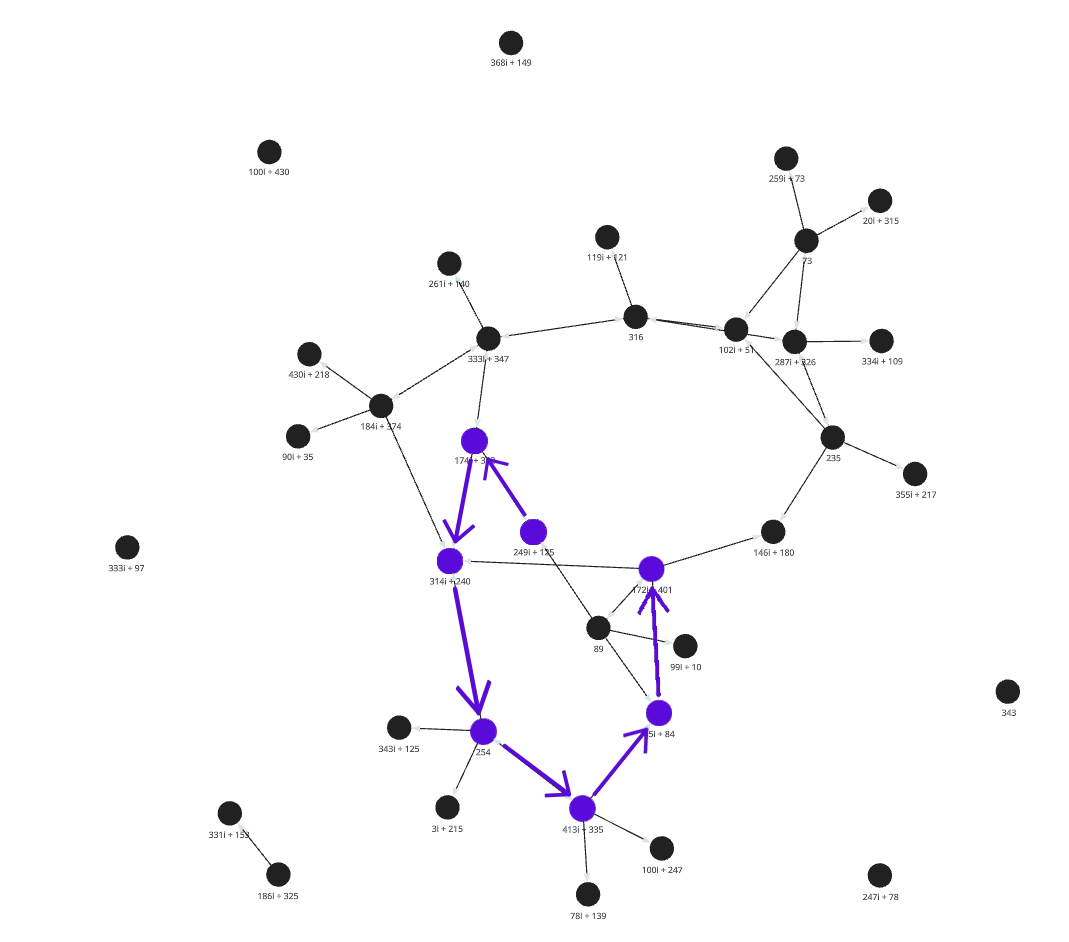
\includegraphics[width=\linewidth]{img/3-isogeny/step6.png}
\caption{Camino final por el grafo de 3-isogenias}
\end{subfigure}
\caption{Caminos finales por los grafos de isogenias para $p=433$}
\label{fig:grafos-final}
\end{figure}

\begin{figure}[!h]
\begin{subfigure}[h]{0.4\linewidth}
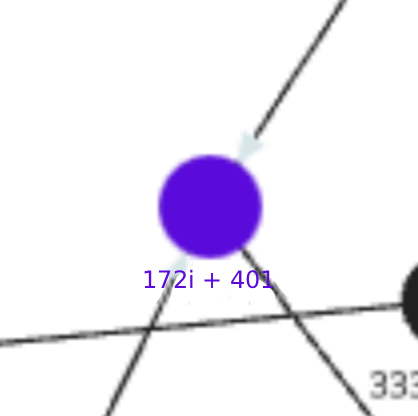
\includegraphics[width=\linewidth]{img/2-isogeny/closeup.png}
\caption{$j$-invariante final en el grafo 2-isogenias}
\end{subfigure}
\hfill
\begin{subfigure}[h]{0.4\linewidth}

\includegraphics[width=\linewidth]{img/3-isogeny/closeup.png}
\caption{$j$-invariante final en el grafo 3-isogenias}
\end{subfigure}
\caption{$j$-invariante final en los grafos.}
\label{fig:grafos-invariante}
\end{figure}


\subsubsection{Implementación}

A la hora de simular este intercambio de clave para llegar al secreto compartido, hemos seguido los pasos proporcionados por los desarrolladores de la implementación Java \cite{sike-java}. A continuación, proporcionaremos el código exacto para los pasos que hemos explicado anteriormente.

El proceso de encapsulación comienza con Bob generando una clave. Tenemos a elegir entre los cuatro conjuntos de parámetros predefinidos y una implementación optimizada o una de referencia. Vamos a utilizar la implementación optimizada dado que no vamos a tratar con el código fuente sino que vamos a utilizarlo, nos interesa más la rapidez que la legibilidad del código.

\begin{verbatim}
SikeParam sikeParam = new SikeParamP434(ImplementationType.OPTIMIZED);
KeyGenerator keyGenerator = new KeyGenerator(sikeParam);
KeyPair keyPairB = keyGenerator.generateKeyPair(Party.BOB);
\end{verbatim}

A continuación comienza el proceso de intercambio de claves propiamente dicho. Alice genera su paso intermedio, la entidad \verb|sike|, y, con la clave pública de Bob, la encapsula.

\begin{verbatim}
Sike sike = new Sike(sikeParam);
EncapsulationResult encapsulationResult 
    = sike.encapsulate(keyPairB.getPublic());
\end{verbatim}

Alice calcula el secreto compartido, la curva final, y el mensaje cifrado.

\begin{verbatim}
byte[] secretA = encapsulationResult.getSecret();
EncryptedMessage encryptedMessage 
    = encapsulationResult.getEncryptedMessage();
\end{verbatim}

Bob recibe el mensaje cifrado \verb|encryptedMessage| como un array de bytes y utiliza la clave pública para el descifrado, obteniendo así su clave secreta. 

\begin{verbatim}
byte[] encodedMessage = encryptedMessage.getEncoded();
EncryptedMessage transportedMessage 
    = new EncryptedMessage(sikeParam, encodedMessage);
byte[] secretB = sike.decapsulate(
                    keyPairB.getPrivate(), 
                    keyPairB.getPublic(), 
                    transportedMessage
                );
\end{verbatim}

Ahora tenemos dos secretos, los correspondientes a Alice y Bob, \verb|secretA| y \verb|secretB| respectivamente. La implementación proporcionada por Wultra funciona de manera correcta y estos dos secretos efectivamente coinciden. Sin embargo, en nuestro proyecto, para añadir una capa de seguridad extra, comprobamos que estos dos coincidan antes de continuar con el cifrado del mensaje.

%
% CIFRADO
%

\subsection{Cifrado}

Una vez tenemos el secreto compartido, veamos cómo funciona el cifrado con SIKE.

\begin{enumerate}
    \item \textbf{Preparación}: se establecen los parámetros públicos, esto es, los parámetros comentados en el apartado anterior, además de la familia de funciones resumen $\mathcal{H} = \{ H_k : k \in K \}$, donde $K$ es un conjunto finito y cada $H_k$ es una función resumen distinta. SIKE no utiliza una función resumen reconocida como SHA-3, sino que incluye un elemento de variabilidad en el cifrado al tener esta familia de funciones y para cada cifrado elegir una diferente de manera pseudo-aleatoria.
    
    \item \textbf{Generación de la clave}: seguimos el protocolo de intercambio de clave de donde obtenemos
    \begin{itemize}
        \item La clave pública $(E_A, \{ P_A, Q_A \})$
        \item Un elemento secreto pseudo-aleatorio $k$
        \item La curva $E_{AB}$ compartida.
    \end{itemize}

    \item \textbf{Cifrado}: el cifrado de SIKE consiste en una multiplicación lógica. Para ello, antes de nada, calculamos el $j$-invariante de la curva compartida $E_{AB}$
        \[ j = j(E_{AB}) \]
    del que calculamos el resumen utilizando una función resumen perteneciente a la familia $\mathcal H$ escogida pseudo-aleatoriamente. Es por esto por lo que un elemento $k \in K$ forma parte de la clave privada. 
        \[ h = H_k(j) \]
    una vez ya tenemos calculado el resumen del $j$-invariante, hacemos la multiplicación lógica con el mensaje en claro $m$ para obtener el mensaje cifrado $c$
        \[ c = h \oplus m \]

    \item \textbf{Descifrado}: como tanto el elemento $k$ como la curva $E_{AB}$ forman parte del secreto compartido, para conseguir el texto en claro a partir del texto cifrado tan solo tenemos que deshacer los pasos del cifrado. Calculamos $j$ y $h$ igual que antes
        \[ j = j(E_{AB}), \, h = H_k(j) \]
    y luego simplemente calculamos la multiplicación lógica del mensaje cifrado $c$ para encontrar $m$
        \[ m = h \oplus c \]
\end{enumerate}

Como podemos ver, el cifrado es simplemente una multiplicación lógica, la seguridad del cifrado reposa íntegramente sobre la dificultad de computar el secreto compartido.

\subsubsection{Implementación}

A la hora de implementar el cifrado, hemos simplificado la elección de la función hash. En vez de generarla pseudo-aleatoriamente con un parámetro $k$ perteneciente a la clave pública, utilizamos siempre la misma, una instancia de \verb|SHAKE256|, derivada de SHA-3. A continuación, analizamos el funcionamiento del método implementado.

En primer lugar, a partir del mensaje original o $m$, generamos el array de bytes que lo representa.

\begin{verbatim}
public byte[] encode(SikeEntity sikeEntity) {
    String message = sikeEntity.getOriginalMessage();
    byte[] messageBytes = message.getBytes(StandardCharsets.UTF_8);
\end{verbatim}

A continuación, creamos una instancia \verb|SHAKE| y la actualizamos con el secreto compartido, es decir, hacemos el hash del secreto compartido.

\begin{verbatim}
    SHAKEDigest shake = new SHAKEDigest(256);
    byte[] keyBytes = sikeEntity.getKeyBytes();
    shake.update(keyBytes, 0, keyBytes.length);
\end{verbatim}

Una vez tenemos los dos arrays de bytes, generamos el mensaje cifrado o $c$ haciendo la multiplicación lógica de estos dos.

\begin{verbatim}
    byte[] encodedMessage = new byte[messageBytes.length];
    for (int i = 0; i < messageBytes.length; i++) {
        encodedMessage[i] = (byte) (keyBytes[i%16] ^ messageBytes[i]);
    }
\end{verbatim}

Este producto final, es el mensaje cifrado que devolvemos.

\begin{verbatim}
    return encodedMessage;
}
\end{verbatim}

El método que calcula el mensaje en claro es idéntico al anterior, la única diferencia es que en vez del mensaje original utilizamos el mensaje cifrado que acabamos de calcular y en vez de devolver el array de bytes del mensaje cifrado, devolvemos un \verb|String| con el mensaje en claro final.

\begin{verbatim}
public String decode(SikeEntity sikeEntity) {
    byte[] encodedMessage = sikeEntity.getEncodedMessage();

    SHAKEDigest shake = new SHAKEDigest(256);
    byte[] keyBytes = sikeEntity.getKeyBytes();
    shake.update(keyBytes, 0, keyBytes.length);

    byte[] decodedMessageBytes = new byte[encodedMessage.length];
    for (int i = 0; i < encodedMessage.length; i++) {
        decodedMessageBytes[i] = (byte) (keyBytes[i%16] 
                                    ^ encodedMessage[i]);
    }

    return new String(decodedMessageBytes);
}
\end{verbatim}

Al igual que en la fase de intercambio de llaves no es realmente necesario comprobar que el secreto compartido se haya calculado correctamente pero igualmente lo hacemos. A la hora de cifrar y descifrar el mensaje también incluimos una comprobación de que todo ha ido correcto.

%
% SEGURIDAD
%

\section{Seguridad}

Al contrario que la criptografía de curvas elípticas clásica, SIDH no se basa en el problema del logaritmo discreto, sino en un problema de complejidad clásico llamado "claw finding problem" (poblema de la pinza, de aquí en adelante) que, en vez de buscar una factorización, busca dos funciones con un mismo valor en dos puntos cualesquiera.

\begin{definition}[Oráculo cuántico estándar]
    En un entorno cuántico, un oráculo de dos funciones $f,g$ se define como
    \[ O_{f,g}: |p,z,w\rangle \to |p,z\oplus P(p)\,\,(\,\text{mod} |Z|\,),w\rangle \]
    donde $p\in W\cup Y, z\in Z,w$ es el espacio de trabajo, y
    \[ P(p) = \begin{cases}
       f(p) &\text{si } p \in X \\
       g(p) &\text{si } p \in Y
    \end{cases} \]
\end{definition}

\begin{problem}[Problema de la pinza]
    Dadas dos funciones $f:X:=[N] \to Z$ y $g:Y:=[M] \to Z$ mediante un oráculo con $N \geq M$ y $Z=[\,|Z|\,],$ encontrar un par $(x,y) \in X \times Y$ para los cuales $f(x) = g(Y)$, si existe. \cite{claw-finding-algorithms}
\end{problem}

Este problema, en vez de tratar con la propia curva trata con la interacción entre curvas.

\begin{table}[!ht]
    \centering
    \begin{tabular}{ |p{0.25\linewidth}||p{0.33\linewidth}|p{0.33\linewidth}|}
        \hline
        & ECDH & SIDH \\
        \hline
        Elementos & Puntos de la curva & $j$-invariante \\
        Computación & $k,P \to [k]P$ & $\phi,E \to \phi(E)$ \\
        Secreto & Escalar $k$ & Isogenia $\phi$ \\
        Problema & Logaritmo discreto & Problema de la pinza \\
        \hline
    \end{tabular}
    \caption{Comparación con la criptografía clásica de curvas elípticas}
    \label{tab:ecdh-vs-sidh}
    \cite{sidh-sike}
\end{table}

Cuando primero se ideó SIKE, el mejor ataque contra el protocolo era atacar directamente el problema de la pinza, lo que conlleva complejidad $O(p^{1/4})$ en un contexto clásico y $O(p^{1/6})$ en uno cuántico. Esto permitía tener una gran seguridad con una clave pública bastante pequeña. SIKEp751, la propuesta de mayor tamaño de SIKE, tiene una clave pública de 564 bytes mientras que McEliece, otro protocolo propuesto, tiene el mismo nivel de seguridad, el máximo que otorga el NIST, pero con una clave pública de 1044992 bytes. 

%
% DESCALIFICACIÓN DEL NIST
%

\section{Descalificación del NIST}\label{sec:estudioteorico:descalificacion}

Como ya hemos mencionado en varias ocasiones, SIKE ha sido descalificado del NIST al haberse encontrado un ataque clásico no genérico que explota los puntos auxiliares para encontrar un camino alternativo a la curva compartida secreta.

Este ataque publicado no fue el primer acercamiento al diseño de un ataque no genérico contra SIDH. En 2017, Petit publicó un algoritmo que permitía encontrar el secreto para algunos casos particulares de SIDH \cite{petit}, sin embargo, el protocolo de forma general y SIKE en particular todavía se consideraban seguros.

El ataque publicado el 22 de julio de 2022 por Castryck y Decru \cite{efficient_attack} permitía, en ese momento, romper SIKEp434 en una hora y SIKEp751, el primo más grande contemplado por SIKE con el nivel más alto de seguridad, en unas 20 usando un ordenador de núcleo único. 

Dado al atractivo de SIKE por su pequeño tamaño de clave y de texto cifrado se intentó en un primer momento salvar a SIDH aumentando el tamaño de los parámetros.  Entre otras propuestas encontramos \textit{Masked-degree SIDH} \cite{masked-degree-sidh} y \textit{SIDH with masked torsion point images} \cite{masked-torsion-sidh}. Lamentablemente, con mejoras posteriores los tiempos del ataque eficiente se reducen a menos de un minuto y menos de una hora, por lo que SIKE fue finalmente descalificado.

La caída en desgracia de SIKE no termina ahí, ya que sigue existiendo SIDH que, como hemos visto, es la generalización de la propuesta al NIST. No obstante, ese mismo año en agosto, Maino y Martindale publican \textit{An attack on SIDH with arbitrary starting curve} que generaliza el ataque de Castryck y Decru a cualquier esquema de SIDH que publique los puntos auxiliares.
     \chapter{Metodología}\label{metodologia}

En esta sección repasaremos cómo hemos dividido y organizado las 300 horas de desarrollo del proyecto. Trataremos tanto las fases de preparación e introducción así como el desarrollo en sí y su verificación y repaso.

\section{Fases del desarrollo}

\begin{figure}[h]
    \centering
    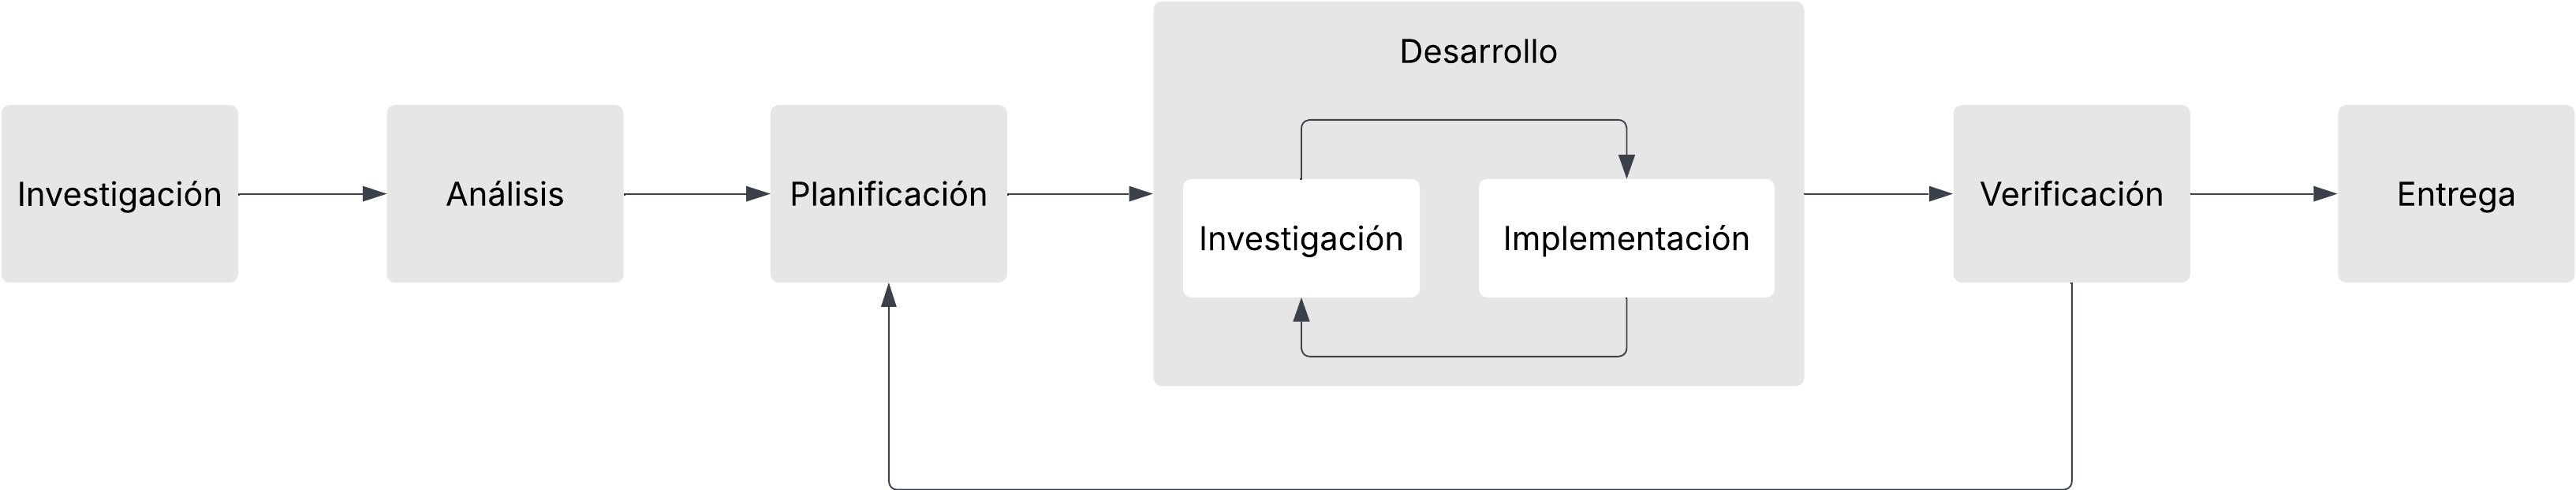
\includegraphics[width=1\linewidth]{img/metodologia.png}
    \caption{Fases del desarrollo}
    \label{fig:metodologia}
\end{figure}

\subsection{Investigación}

Dado que la criptografía post-cuántica en general, y SIKE con su base matemática en isogenias es un tema complejo que no habíamos tratado previamente, decidimos empezar investigando para comenzar el desarrollo con, al menos, una visión general del protocolo.

El artículo principal que hemos tratado ha sido la presentación de de Feo, Jao y Plût al NIST \cite{towards_quantum_resistant_cryptosystems}. Sin embargo, debido a la alta complejidad matemática, hemos tenido que dar varios rodeos antes de poder centrarnos en él y realmente interiorizarlo.

Algunos de los temas que hemos tenido que estudiar son curvas elípticas, sobre todo las consideradas supersingulares, isogenias y $j$-invariantes. Todos estos temas se ven reflejados en el capítulo \ref{conceptosprevios}, de Conceptos Previos.

\subsection{Análisis}

Una vez tuvimos una idea general del protocolo y de sus bases, nos sentimos ya preparados para hacer un primer esquema del qué y el cómo íbamos a hacer. Incluye tanto la realización de un primer esquema de la memoria como el de la interfaz gráfica.

Esta fase es la más corta ya que tan sólo consiste en una vista general de la organización, no una planificación concreta.

\subsection{Planificación}

Una vez definido el objetivo final general con una visión específica de qué había que redacar y/o implementar, desmigamos el proceso para comenzar el desarrollo del proyecto de una forma razonable y eficaz.

Durante este primer proceso de planificación, definimos las actividades principales así como sus componentes, en caso de considerarlo necesario. Se clasifican estas tareas por su dominio (memoria, frontend o backend) y por su prioridad (crítica, alta, media, baja y opcional).

La planificación no sólo se queda aquí, conforme empezamos a desarrollar, nos encontramos incidencias que debemos manejar. De esta forma el trío planificación-desarrollo-verificación forma un bucle sobre el que iteraremos a lo largo del desarrollo del proyecto.

\subsection{Desarrollo}

Durante la fase de desarrollo estamos trabajando en el proyecto de manera efectiva, ya sea escribiendo parte de la memoria o la implementación gráfica. Esta fase tiene sus propias fases internas de investigación y desarrollo/implementación de parte de la interfaz gráfica. En general hemos trabajado con tecnologías que conocíamos, sin embargo, siempre hay innovaciones y mejoras que debemos probar y verificar a lo largo de un proyecto software, por pequeño que sea.

\subsection{Verificación}

En esta fase, comprobamos que todo vaya correcto. Esto incluye revisiones por parte del tutor así como pruebas formales e informales de la interfaz gráfica. Durante esta fase anotamos todo aquello que no ha ido como debería para, volviendo a la fase de planificación, poder crear las nuevas actividades de manera rigurosa.

\subsection{Entrega}

La entrega es la fase final, una vez el proyecto terminado, se procede a la entrega oficial de la memoria y la realización de la presentación y la defensa del proyecto.
     \chapter{Planificación y costes}\label{planificacion}

En esta sección repasaremos la planificación detallada del proyecto, esto incluye una lista completa de actividades así como un desglose de horas.

\section{Listado completo de actividades}

\renewcommand{\arraystretch}{1.5}
\begin{longtable}{|p{0.03\linewidth}|p{0.52\linewidth}|p{0.105\linewidth}|p{0.1\linewidth}|p{0.1\linewidth}|}

    % cabecera
    \hline \textbf{Id} & \textbf{Descripción} & \textbf{Ámbito} & \textbf{Prioridad}  & \textbf{Horas}\\ \hline \endhead
    
    % memoria
    1 & Lectura y comprensión del artículo principal & Memoria & Crítica & 7.5 \\ \hline
    2 & Consulta de artículos matemáticos de soporte para aclarar y completar ideas & Memoria & Crítica & 15 \\ \hline
    3 & Consulta de artículos relacionados con SIKE de soporte para aclarar y completar ideas & Memoria & Crítica & 5 \\ \hline
    4 & Desarrollo de un índice primitivo & Memoria & Alto & 0.5 \\ \hline
    5 & Redacción de las secciones matemáticas de la memoria & Memoria & Medio & 45 \\ \hline
    6 & Redacción de las secciones criptográficas de la memoria & Memoria & Medio & 45 \\ \hline
    7 & Redacción de las secciones técnicas de la memoria & Memoria & Medio & 45 \\ \hline
    8 & Correcciones y cambios tras revisiones propias y/o del tutor (incluye tutorías) & Memoria & Alto & 20 \\ \hline
    9 & Preparación de la presentación y estudio & Memoria & Alto & 3 \\ \hline

    % frontend
    10 & Idea general de la distribución de la interfaz & Frontend & Crítico & 0.5 \\ \hline
    11 & Vista de inicio & Frontend & Medio & 5 \\ \hline
    12 & Menú de protocolos & Frontend & Medio & 1.5 \\ \hline
    13 & Página de información & Frontend & Bajo & 1.5 \\ \hline
    14 & Vista de presentación de protocolo & Frontend & Crítico & 10 \\ \hline
    15 & Presentación del protocolo de prueba de identidad & Frontend & Bajo & 5 \\ \hline
    16 & Presentación del protocolo de intercambio de llave & Frontend & Alto & 15 \\ \hline
    17 & Presentación del protocolo de cifrado & Frontend & Alto & 20 \\ \hline
    18 & Conexión con el backend y contexto & Frontend & Alto & 7.5 \\ \hline
    19 & Correcciones de estilo en función del tamaño de la pantalla & Frontend & Bajo & 5 \\ \hline
    20 & Internacionalización de la interfaz & Frontend & Bajo & 5 \\ \hline
    21 & Diseñar e implementar el conjunto de pruebas & Frontend & Medio & 10 \\ \hline

    % backend
    22 & Diseño de la entidad base en función de las necesidades de la interfaz y el funcionamiento de la implementación de SIKE & Backend & Crítico & 0.5 \\ \hline
    23 & Implementar entidad y builder & Backend & Alto & 5 \\ \hline
    24 & Implementar capa de servicio & Backend & Alto & 1 \\ \hline
    25 & Implementar controladores & Backend & Alto & 1 \\ \hline
    26 & Modificar seguridad por defecto del proyecto Spring para el acceso a los endpoints & Backend & Alto & 5 \\ \hline
    27 & Diseñar e implementar el conjunto de pruebas & Backend & Medio & 10 \\ \hline

    % otros: soporte, despliegue, etc
    28 & Investigación y consulta para resolver problemas de implementación específicos & Soporte & Bajo & 25 \\ \hline
    29 & Investigación de medios y plataformas de despliegue disponibles & Despliegue & Alto & 5 \\ \hline
    30 & Despliegue y resolución de incidencias inmediatas relacionadas & Despliegue & Alto & 3 \\ \hline
    & TOTAL &&& 300 \\ \hline
    
    \caption{Listado completo de actividades y sus características}
    \label{tab:actividades}
\end{longtable}

\section{Cronograma}

En esta sección compararemos el trabajo planificado y lo compararemos con el trabajo real realizado.

\subsection{Estimación original}

En la figura \ref{fig:cronograma-original} tenemos la planificación original del proyecto. 


\subsection{Cronograma final y desviación}

En la figura \ref{fig:cronograma-real} tenemos el cronograma final del proyecto. 

La primera gran diferencia es la misma escala temporal, nuestra idea era presentarnos a la primera convocatoria. Una vez comenzamos a trabajar, vimos que la dedicación necesaria era mayor a la esperada y cada fase del proyecto se alargó. Las primeras fases, las de investigación y redacción de la memoria, son prácticamente idénticas si ignoramos la diferencias de fechas.

A la hora de la implementación gráfica si ha habido más desorden en comparación con la planificación original. El backend, que era lo primero que estaba previsto hacer, lo atrasamos hasta ya tener el frontend montado y la conexión con el frontend no lo hicimos una vez la aplicación estaba iniciada sino una vez realizamos el protocolo de cifrado.

El desarrollo del frontend siguió la planificación original (salvo a la hora de realizar cada uno de los protocolos, aunque este cambio no es relevante realmente) en mayor parte porque esta planificación seguía el orden lógico de interacción con la página.


\begin{landscape}
\begin{figure}[!ht]
    \centering
    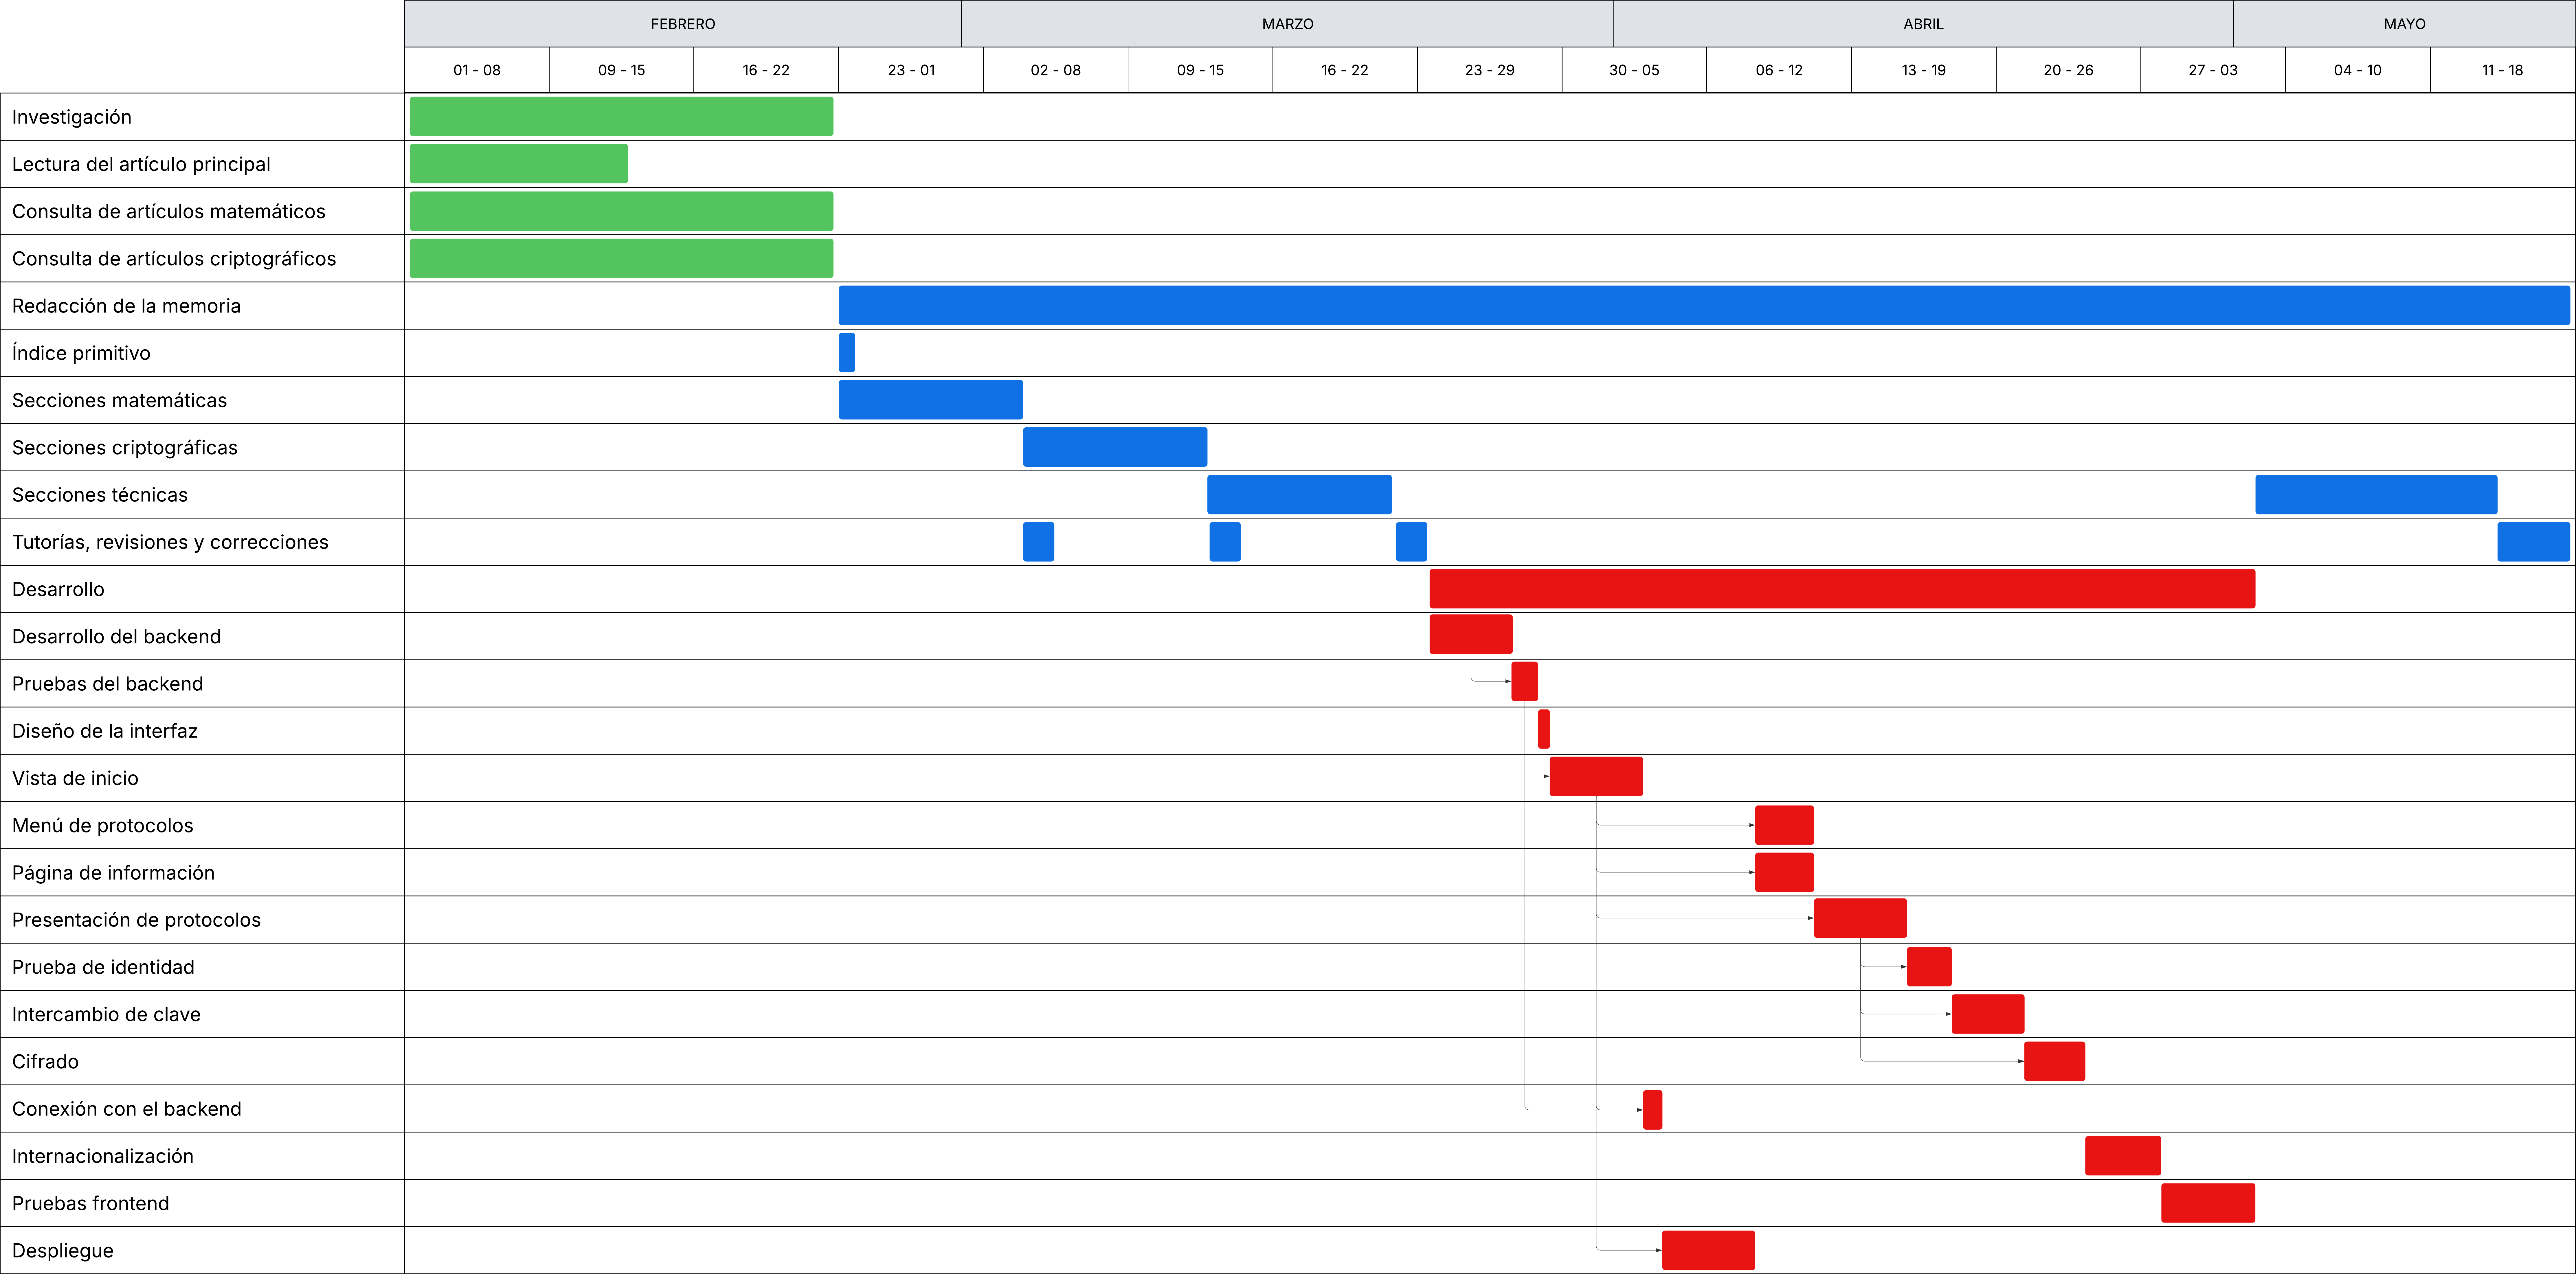
\includegraphics[width=\linewidth]{img/cronograma-original.png}
    \caption{Cronograma original}
    \label{fig:cronograma-original}
\end{figure}
\end{landscape}

\begin{landscape}
\begin{figure}[!ht]
    \centering
    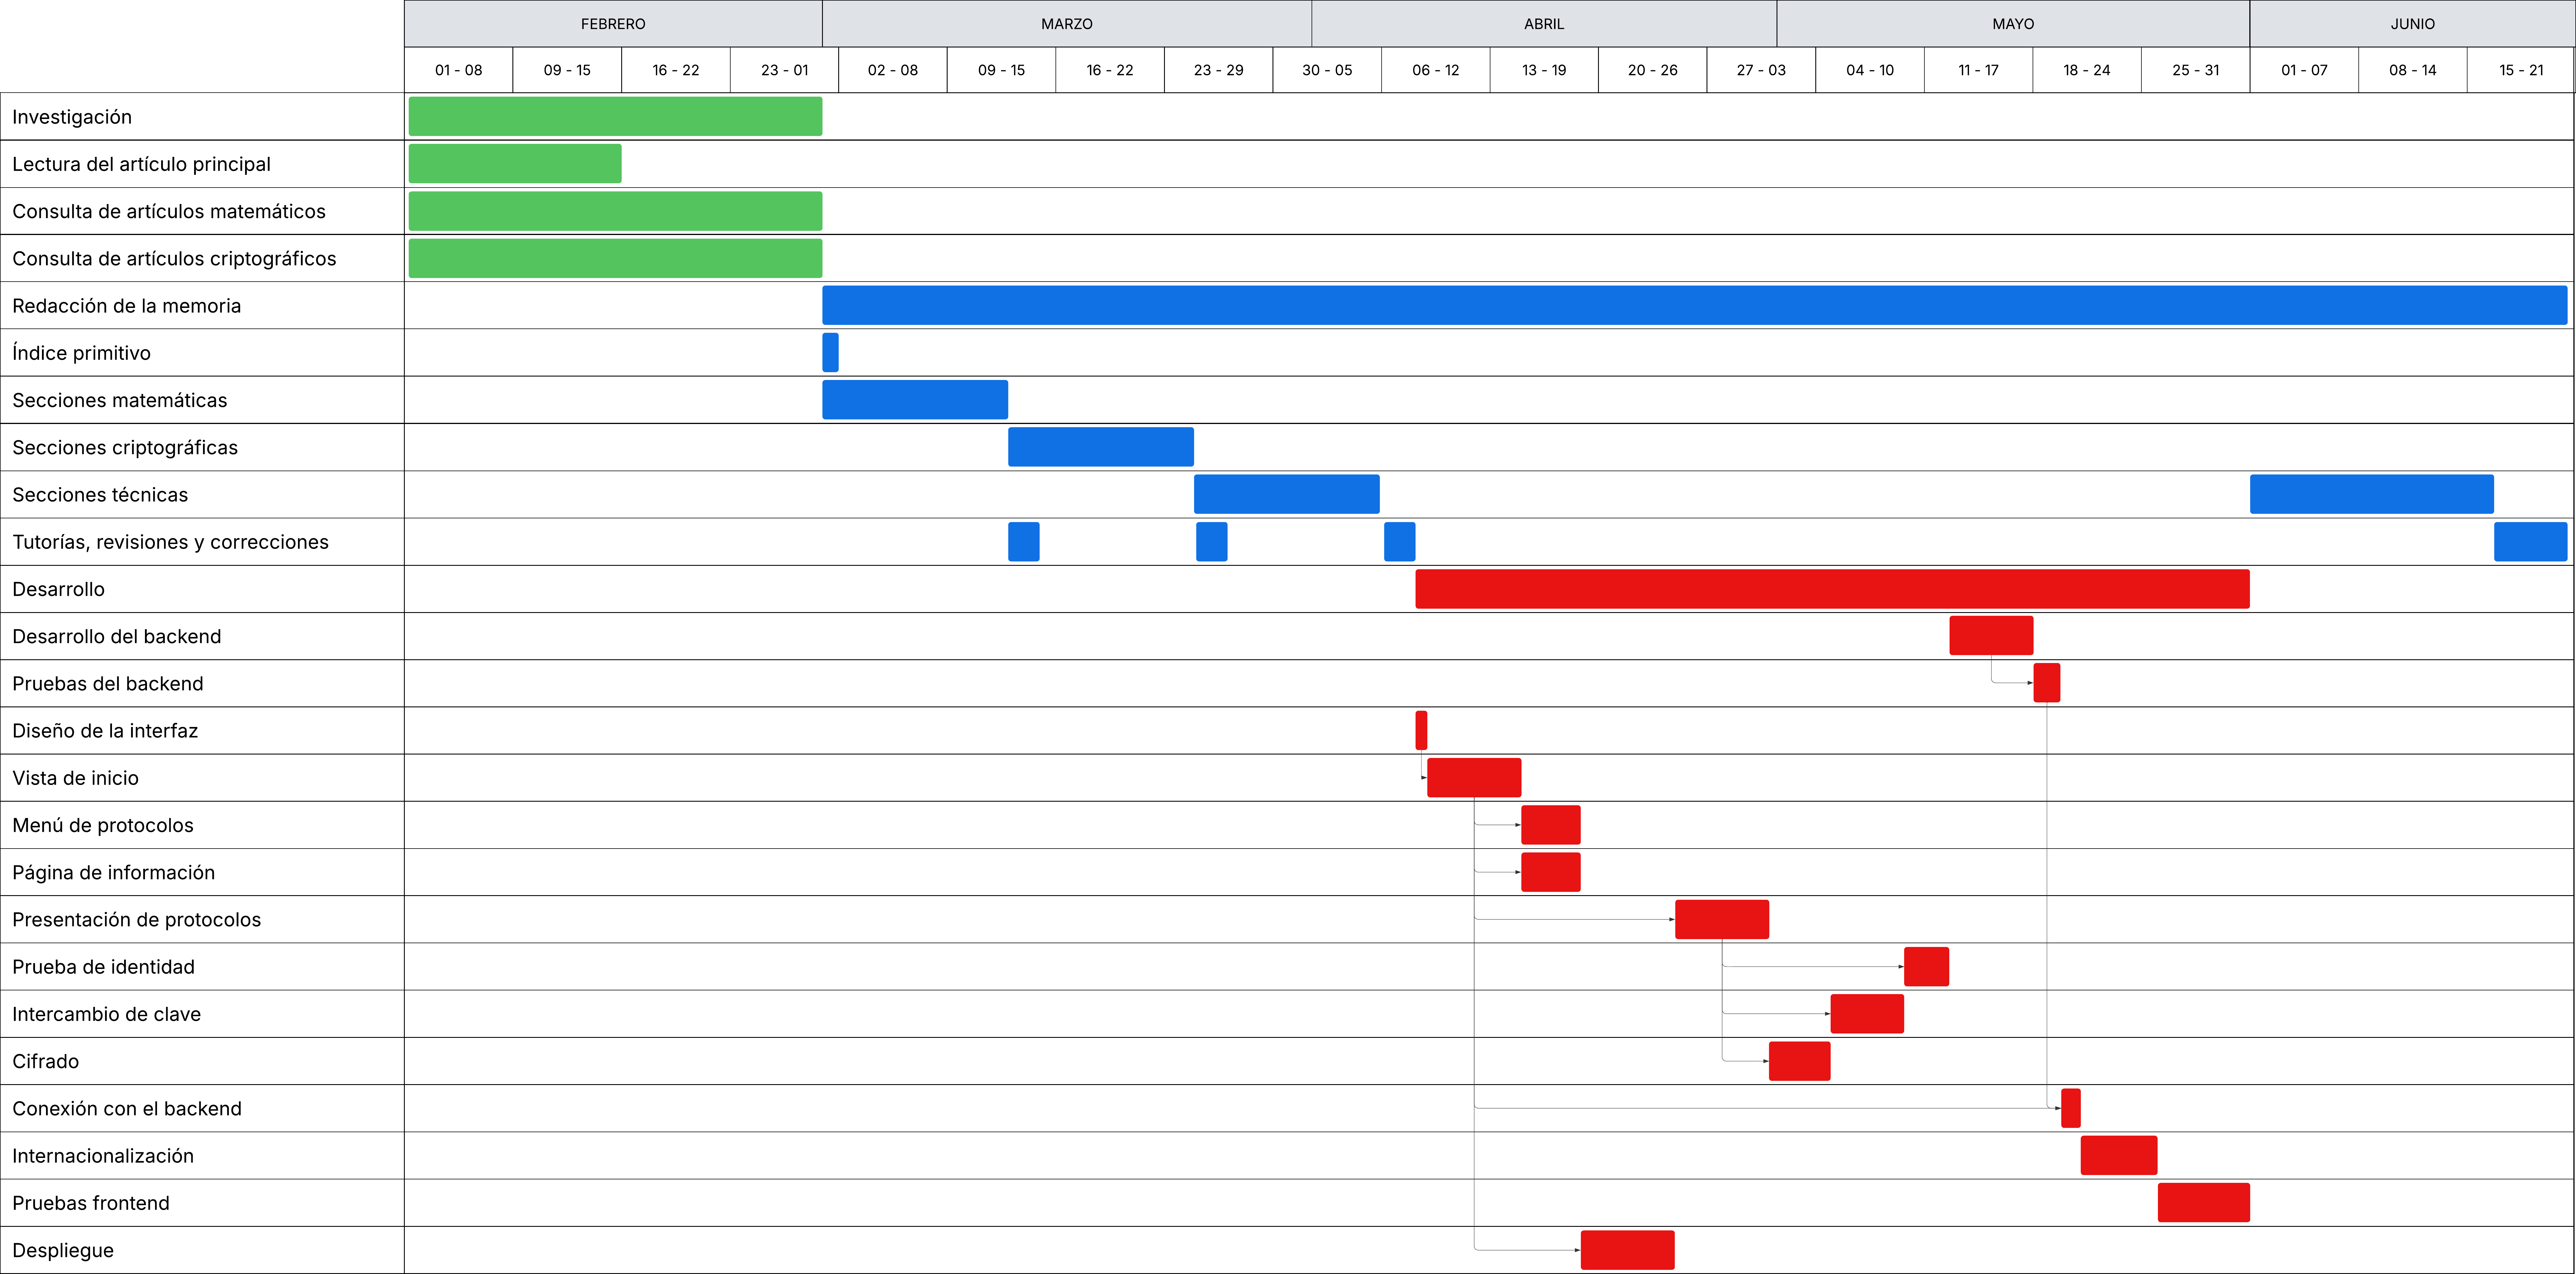
\includegraphics[width=\linewidth]{img/cronograma-real.png}
    \caption{Cronograma real}
    \label{fig:cronograma-real}
\end{figure}
\end{landscape}



\section{Costes}

Para calcular un coste total estimado del proyecto, utilizaremos la fórmula del Total Cost of Ownership o TCO, que contempla tanto gastos de capital como gastos operativos.

Los gastos de capital o CapEx incluyen los gastos materiales como son el ordenador y otros aparatos tecnológicos que se hayan utilizado. Los gastos operativos o OpEx incluyen los costes del personal así como los costes de licencias software que se hayan utilizado.

No se considerarán otros costes relacionados con la electricidad o la conexión a internet al no poder determinar con seguridad su impacto en el desarrollo del proyecto.

Una vez tengamos los costes de capital y operativos calculados, podremos calcular el TCO como

\[ TCO = CapEx + OpEx \]

Sin embargo la estimación no se termina ahí ya que este se considera el coste base del proyecto, hay que tener en cuenta los márgenes de contingencia, el beneficio y el IVA.


\begin{table}[!ht]
    \centering
    \begin{tabular}{ccc}\toprule
         \textbf{Concepto}&  \textbf{Porcentaje}& \textbf{Fórmula}\\\midrule
         Márgenes de contingencia& $10\%$&$0,1 \cdot TCO$\\
         Beneficio& $10\%$&$0,1 \cdot TCO$\\ \hline
         \textbf{Subtotal}& &$0,2 \cdot TCO$\\ \hline
         IVA (21\%)& $21\%$&$0.21 \cdot Subtotal$\\ \hline
         \textbf{Total}&  & $Subtotal + IVA$\\ \bottomrule
    \end{tabular}
    \caption{Coste final una vez calculado el TCO}
    \label{tab:formulas-TCO}
\end{table}

\subsection{Costes de capital}

Como costes de material del proyecto contamos la amortización del ordenador utilizado para el desarrollo: un portátil MSI Prestige 15 A12USCX con un valor de mercado aproximado de 1100€.

Según la Agencia Tributaria, los sistemas informáticos se pueden amortizar con un coeficiente lineal máximo del 26\% \cite{agencia-tributaria-amortizacion}. Considerando un desarrollo aproximado de 5 meses, el coste lo hemos calculado como

\[ \frac{26}{100} \cdot \frac{5}{12} \cdot 1100 = 119,17 €  \]

No vamos a considerar más amortizaciones por motivos similares a el porqué no consideramos el coste de las infraestructuras. Esto junto a que el coste material es el único que vamos a considerar en el CapEx, nos resulta en lo siguiente:

\[ CapEx = 119,17 € \]

\subsection{Costes operativos}

\subsubsection{Gastos de personal}

Para el cálculo de los costes de personal tomamos como referencia el informe de mercado de perfiles informáticos realizado por la Consejería de Agricultura, Pesca y Desarrollo Rural de la Junta de Andalucía \cite{precios}. Dado que se trata de un trabajo fin de grado, consideraremos los perfiles Junior para todos los roles.

A partir del listado de tareas en la sección anterior, haremos la siguiente división de horas que equivaldrá al correspondiente coste.

\begin{table}[!ht]
    \centering
    \begin{tabular}{ccll}\toprule
        \textbf{Rol}& \textbf{Horas}& \textbf{Tarifa (€/h)}&\textbf{Coste}\\\midrule
        Jefe de proyecto& 50& 39,16&1.958\\
        Desarrollador&  121.5& 24,10&2.928,15\\
        Tester de calidad&  20& 23,77&475,4\\ \hline
        \textbf{Total}& 191,5& &5.361,65\\ \bottomrule
    \end{tabular}
    \caption{Coste de personal estimado}
    \label{tab:coste-personal}
\end{table}

\subsubsection{Software y licencias}

Dado que todas las herramientas que hemos utilizado a lo largo del proyecto han sido gratuitas (GitHub, Render, Overleaf) no consideramos los costes. Finalmente, obtenemos los siguientes gastos operativos estimados:

\[ OpEx = 5.361,65 € \]

\subsection{Estimación final}

Una vez calculados el CapEx y el OpEx, podemos calcular el TCO como base de los costes del proyecto.

\[ TCO = CapEx + OpEx = 119,17 + 5.361,65 = 5480,82 \]

Utilizamos la tabla \ref{tab:formulas-TCO} para hacer las estimaciones finales.\footnote{Se ha realizado un redondeo a dos cifras decimales.}

\begin{table}[!ht]
    \centering
    \begin{tabular}{cc}\toprule
        \textbf{Concepto}& \textbf{Coste estimado}\\\midrule
        Márgenes de contingencia&$548,08$\\
        Beneficio&$548,08$\\ \hline
        \textbf{Subtotal}&$6.576,98$\\ \hline
        IVA (21\%)&$1.381,17$\\ \hline
        \textbf{Total}& $7.958,15$\\ \bottomrule
    \end{tabular}
    \caption{Coste final una vez calculado el TCO}
    \label{tab:calculo-TCO}
\end{table}
     \chapter{Alcance del proyecto}\label{alcance}

\section{Objetivo}

Este proyecto está pensado para servir de iniciación e introducción a una de las propuestas del NIST, Super-Singular Key Exchange o SIKE. Este protocolo toma de punto de inicio las curvas elípticas supersingulares y adapta los protocolos de Diffie-Hellman y Elgamal con la intención de proporcionar la seguridad necesaria para afrontar los desafíos de la informática postcuántica.

Los objetivos de este trabajo son, pues:

\begin{itemize}
    \item Definir claramente todos aquellos conceptos matemáticos algo más avanzados que utiliza SIKE.
    \item Explicar el protocolo de manera sencilla para facilitar la comprensión de este.
    \item Proporcionar una interfaz que gráficamente muestre cómo funciona el protocolo.
\end{itemize}



\section{Funcionalidades}

El sitio contará con las siguientes funcionalidades:

\begin{itemize}
    \item Explicación paso a paso de cada protocolo.
    \item Enlaces de interés a algunos de los recursos más importantes.
\end{itemize}

\section{Diseño}

El proyecto estará diseñado únicamente para ordenadores debido a los objetivos del mismo y al gran número de partes móviles que este contiene. Para más información técnica, dirigirse al apartado \ref{tecnologias} Tecnologías.

\section{Plazos}

Al ser un Trabajo Fin de Grado del departamento de Matemáticas Aplicadas I, el plazo final de entrega será el 21 de junio de 2026.

\section{Entregables}

Los entregables finales del proyecto serán

\begin{itemize}
    \item \href{https://introduction-to-sike.vercel.app}{Sitio web activo y funcionando}.
    \item Memoria del proyecto (es decir, este documento).
    \item \href{https://github.com/albramvar1/introduction-to-sike}{Código fuente disponible}.
\end{itemize}
     \chapter{Criterios de aceptación}\label{critaceptacion}

Los criterios de aceptación del proyecto son los siguientes

\begin{enumerate}
    \item La página debe ser accesible y funcionar correctamente.
    \item Los conceptos matemáticos deben estar explicados de forma sencilla y cercana.
    \item Debe haber una presentación/explicación para cada uno de los protocolos descritos por SIKE. Estos protocolos son:
    \begin{itemize}
        \item Intercambio de llaves.
        \item Cifrado.
    \end{itemize}
    \item Estas presentaciones serán interactivas, el usuario podrá introducir valores que modificarán los valores calculados.
    \item Se deberá aplicar la implementación real de SIKE para el cálculo de dichos valores.
\end{enumerate}
     \chapter{Análisis de requisitos}\label{requisitos}

Este apartado estudiará los requisitos del sistema, tanto los funcionales como los no funcionales, lo que delimitará el alcance del proyecto con mayor grado de detalle.

\section{Requisitos funcionales}

Describen cómo debe comportarse la aplicación cara al usuario.

\begin{enumerate}
    \item Como usuario de la aplicación, quiero poder visitar la implementación desde la web.

    \item Como usuario, quiero poder ver una explicación de cada parte del protocolo (prueba de identidad cero-conocimiento, intercambio de claves y encriptación/desencriptación).

    \item Como usuario, quiero que estas explicaciones se realicen a través de unas presentaciones que se reproduzcan automáticamente, pero que esta reproducción automática se pause cuando interactúe con ellas.
\end{enumerate}

\section{Requisitos no funcionales}

Describen otras características del proyecto que no implican cambios en el funcionamiento de este.

\subsection{Accesibilidad}

\begin{enumerate}
    \item Como administrador, quiero que la aplicación cumpla los requisitos mínimos de accesibilidad.

    \item Como administrador, quiero el sitio esté disponible tanto en inglés como en español, además de ser fácilmente escalable a la hora de añadir más idiomas.
\end{enumerate}

\subsection{Presentación}

\begin{enumerate}
    \item Como usuario, quiero que el sitio sea responsivo de manera que no tenga demasiados problemas para consultar el sitio sin importar el dispositivo desde donde entre.

    \item Como administrador, quiero que la visualización de los protocolos sólo sea accesible desde ordenadores y/o dispositivos que tengan un mínimo de dimensión, ya que un móvil o similar distorsiona demasiado las proporciones para que se vean con claridad las explicaciones.
\end{enumerate}
     \chapter{Tecnologías}\label{tecnologias}

En este apartado se detallarán las tecnologías, lenguajes y convenciones a las que nos hemos atenido a lo largo de la realización del proyecto.

\section{Backend}

Al estar el proyecto pensado como una interfaz didáctica, el backend es bastante sencillo.

\subsection{Lenguaje informático}

Aunque el ámbito informático es extremadamente amplio y existen siempre miles de alternativas disponibles en cuanto a qué tecnologías usar, en este caso en concreto la decisión ha estado marcada por la necesidad.

Existen tres implementaciones de \href{https://sike.org/}{SIKE según su página oficial}. Una en \href{https://github.com/Microsoft/PQCrypto-SIDH}{C, ofrecida por Microsoft Research}, otra en \href{https://github.com/cloudflare/circl/tree/master/dh/sidh}{Go por Cloudfare} y una última en \href{https://github.com/wultra/sike-java}{Java por Wultra}. De los tres lenguajes mencionados, sólo hemos trabajado con \textbf{Java} por lo que nos decantamos por él.

\subsection{Framework}

Hemos optado por utilizar \textbf{SpringBoot} como framework ya que es el que más hemos utilizado a lo largo de la carrera además de ser seguro y fácilmente escalable.


\section{Frontend}

En el frontend es donde reside la mayor parte del proyecto.

\subsection{Lenguaje informático}

Como lenguaje informático hemos utilizado \textbf{JavaScript} debido a su sencillez y rapidez. Aunque consideramos el uso de TypeScript por su robustez y mayor seguridad, consideramos que, teniendo en cuenta las funcionalidades de la web — esto es, el ser una web casi únicamente de presentación, apenas trata con variables y datos complejos además de tener un gran número de elementos móviles — estas características no eran necesarias y nos interesaba más la inmediatez del JavaScript. 

A la hora de los estilos de la página, consideramos usar Bootstrap con el que hemos trabajado en algunos proyectos. Sin embargo, dado que personalmente siempre me ha entorpecido más que ayudado, decidí utilizar \textbf{CSS} puro, salvo aquellas dependencias que traían sus propios estilos y personalizaciones.

\subsection{Librerías y recursos}

Hemos utilizado \textbf{React} para diseñar el frontend debido a su flexibilidad y a la gran cantidad de componentes ya hechos y listos para su uso. Entre ellos, cabe destacar:

\begin{itemize}
    \item SeraUI (https://seraui.com/): para gran parte de los componentes animados.
    \item Reagraph (https://reagraph.dev/): una librería específica para la visualización de grafos en React.
\end{itemize}


\section{Despliegue y mantenimiento}

Para el despliegue consideramos un gran número de opciones por varios motivos que desglosaremos a continuación.

\subsection{Oracle Cloud}

En primer lugar, intentamos encontrar una forma de desplegar un contenedor docker al completo, ya que el backend es tan mínimo que nos parecía más óptimo el desplegar el proyecto de forma íntegra para evitar exponer el backend y que el mantenimiento fuese lo más cómodo posible.

La mejor opción para ello consistía en utilizar Oracle Cloud, que pone a disposión máquinas virtuales para uso propio que, si se atienen a una serie de restricciones y métricas de uso, pueden ser usados indefinidamente sin coste alguno.

Sin embargo, intentando crear una instancia, nos encontramos con que no hay ninguna disponible en la región que había seleccionado. Como la región no se puede cambiar una vez creada una cuenta, una opción sería empezar a crear cuentas hasta dar con una región que tuviese instancias disponibles. Como cada cuenta necesita un correo diferente y añadir una tarjeta de crédito, no nos pareció buena idea utilizar ese acercamiento.

\subsection{Koyeb}

Según nuestras investigaciones, Koyeb ofrece un único despliegue de forma completamente gratuita, tanto blogs como la misma documentación del sitio. Esta plataforma, además de unas prestaciones bastante buenas, no suspende los despliegues en periodos de baja demanda, como hacen muchas otras plataformas.

Más allá de simple comodidad, este motivo específico me interesaba para desplegar el backend y evitar problemas de funcionamiento del frontend. Podría implementarse un sistema de relevo en el que una vez se arranca el frontend, este haga una llamada de comprobación al backend para asegurarse de que todo está bien o, en el caso de que esté inactivo, que vuelva a arrancar. Por desgracia, este funcionamiento no nos parece suficiente ya que durante todo ese tiempo que el backend tarda en arrancar, el frontend no puede depender de él.

Una opción sería avisar al usuario de la situación, pero teniendo opciones como Koyeb es claramente mejor para el usuario no tener que estar esperando. Desgraciadamente, cuando intentamos crear una cuenta en Koyeb para su uso, este obliga al usuario a pagar una suscripción de 30\$ antes de empezar a usar el sitio, por lo que tuvimos que descartar esta plataforma también.

\subsection{Vercel, Render y Better Slack}

Finalmente, nos decantamos por usar Render, una plataforma que hemos utilizado en varias ocasiones a lo largo de la carrera y es de las pocas que ofrece despliegues gratuitos de contenedores Docker sin mucho problema.

Render, no obstante, sí que implementa la pausa de los servicios si no se detecta un mínimo de actividad. Investigando un poco más, descubrimos que hay plataformas, como Better Slack, que es la que hemos acabado utilizando, que le lanzan una petición HTTP cada cierto tiempo a una dirección cualquiera. 

Poco después nos encontramos con que Render tiene otras restricciones que no conocíamos de antemano que es un máximo total de 750 horas mensuales de los despliegues gratuitos. Es por esto que finalmente hemos decidido desplegar el frontend y el backend por separado, este primero en Vercel que no tiene periodos de suspensión y está centrado para frameworks como React, y el backend en Render, con un monitor que evite su suspensión.
     \chapter{Arquitectura y diseño técnico}\label{disarqtecnica}

\section{Arquitectura de la aplicación}

\begin{figure}[h]
    \centering
    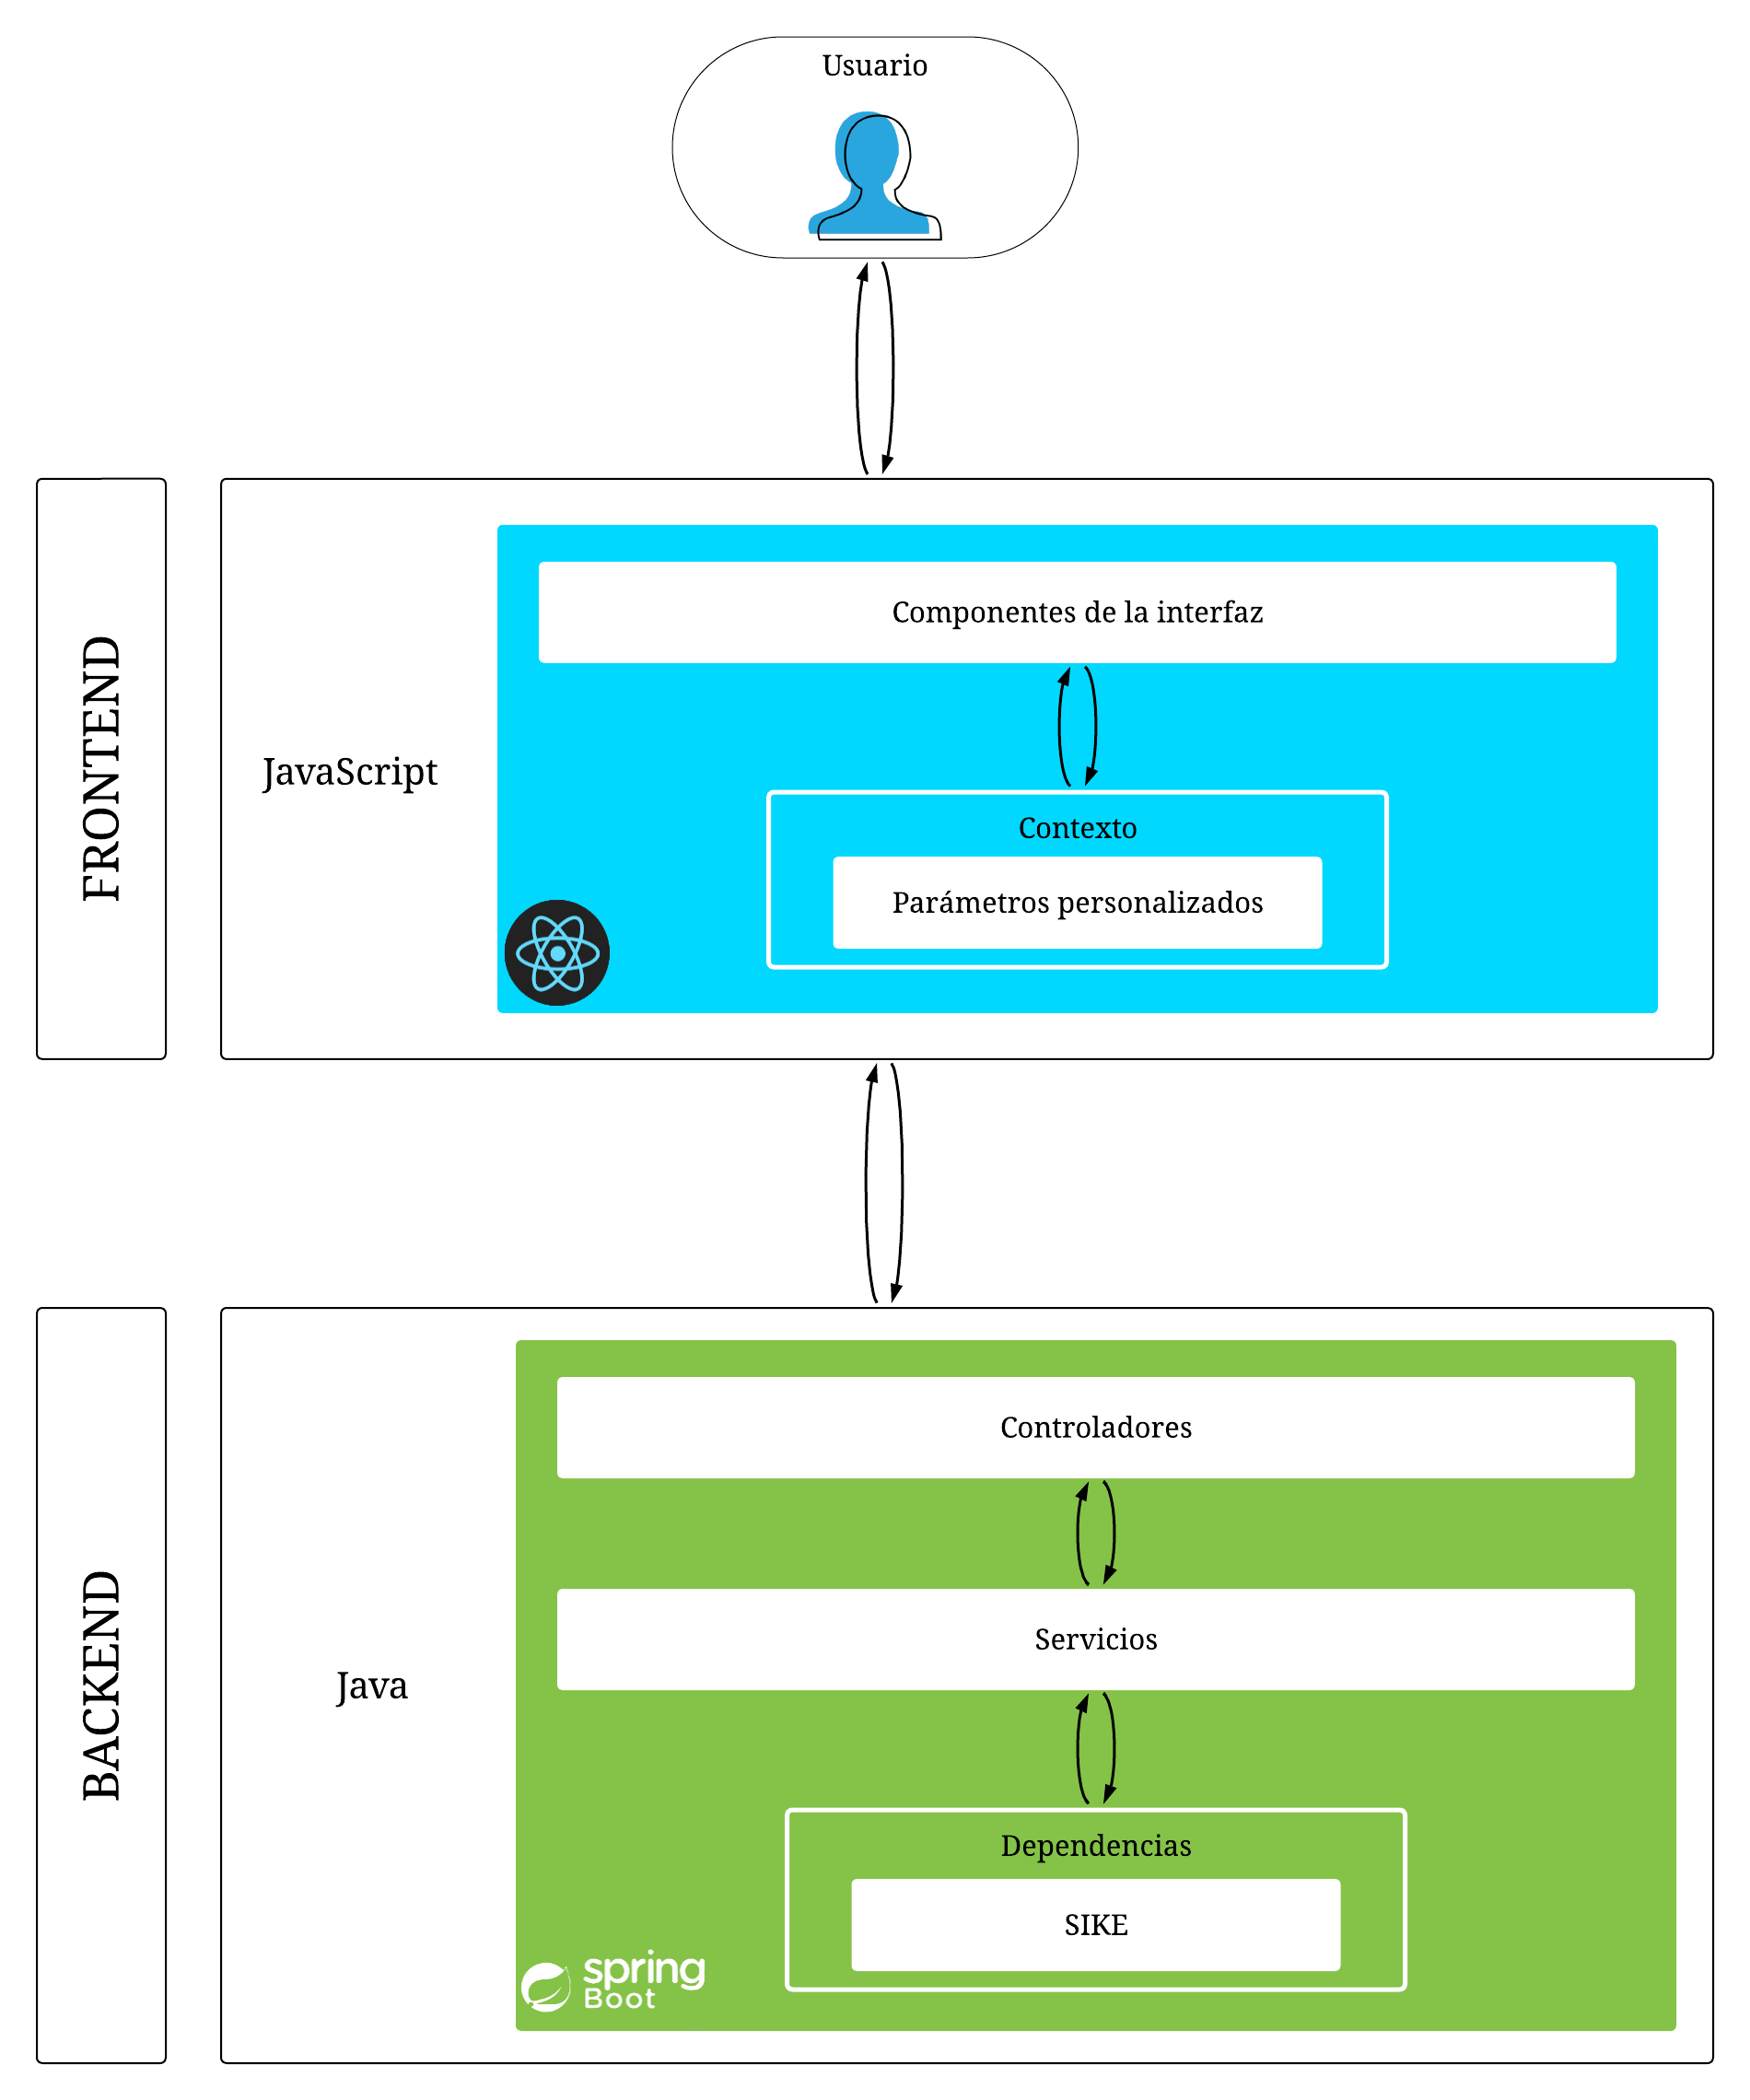
\includegraphics[width=0.75\linewidth]{img/Diagrama de capas.png}
    \caption{Diagrama de la estructura de la aplicación}
    \label{fig:diagrama-capas}
\end{figure}

Puesto que nos hemos visto obligados a utilizar tecnologías diferentes para la capa de presentación y la de lógica, tal y como exponemos en el capítulo \ref{tecnologias} decidimos implementar una arquitectura en capas tal y como queda reflejado en el anterior diagrama.

De esta forma reducimos el acoplamiento y aumentamos la cohesión, al separar las responsabilidades del proyecto. Además, permite utilizar cada capa casi como una unidad independiente.

\section{Diseño de la aplicación}

A continuación, veremos los patrones de diseño que hemos seguido a la hora de desarrollar la aplicación.

\subsection{Patrones creacionales}

En referencia a los patrones utilizados a la hora de crear objetos.

\subsubsection{Builder}

El patrón que hemos utilizado es el de Builder, que permite abstraer la creación de un objeto complejo, como es la entidad sobre la que reposa nuestra implementación, ya que para crear el mensaje cifrado y el mensaje descifrado hace falta lógica específica.

De esta forma conseguimos atomizar el proceso de creación para evitar que cualquier otro proceso del proyecto pueda interferir en él.


\subsection{Patrones estructurales}

En relación a la forma de ordenar internamente el proyecto.

\subsubsection{Module}

A la hora de implementar la vista de presentación de protocolo, en vez de duplicar la lógica de la presentación para cada protocolo, lo que hemos hecho ha sido crear una vista genérica de protocolo \verb|ProtocolView| que llama a las presentaciones específicas. Esta vista general agrupa los componentes marco de las presentaciones, el reproductor y los componentes genéricos inicial y final.

\subsubsection{Objeto Compuesto}\label{objeto-compuesto}

La presentación de los protocolos funciona como una presentación genérica de diapositivas, sin embargo, estas "diapositivas" son componentes React con sus estilos adicionales. Aunque algunas de ellas son tan sencillas como una imagen y algo de texto, hay otras que contienen componentes animados o incluso su propia lógica. Es por esto que decidimos tratar cada protocolo como una presentación al completo, importando a la vista \verb|ProtocolView| previamente definida una lista con todos los componentes para que esta tan sólo itere sobre ella. De esta forma conseguimos simplificar la lógica general a la vez que mantenemos cada paso de la presentación autocontenido.


\subsection{Patrones de comportamiento}

Aquellos que tratan la interacción y responsabilidades entre clases y módulos

\subsubsection{Método Plantilla}

Como hemos mencionado en el patrón \ref{objeto-compuesto} Objeto Compuesto, hay pasos que tienen una lógica interna. Esta lógica queda autocontenida en la subclase y no afecta en ningún momento al reproductor automáticos de las diapositivas.

\subsubsection{Iterador}

Como explicábamos en el patrón de \ref{objeto-compuesto} Objeto Compuesto, tratamos las explicaciones de cada protocolo como una lista de componentes React para simplificar su uso.

\subsubsection{Estado}

Para que los parámetros y valores de ejemplo de SIKE se mantengan constantes a lo largo de la explicación y para que cualquier cambio se refleje a nivel global, utilizamos los contextos que proporciona React, de forma que cuando el usuario introduce un mensaje personalizado o vuelve a generar el secreto compartido, estos valores se reflejen en los pasos siguientes para que el usuario vea una implementación real del protocolo.
     \chapter{Pruebas}\label{pruebas}

\section{Backend}

El backend de la aplicación es extremadamente pequeño, consta de un único endpoint, un método del servicio y las funciones de cifrar y descifrar en la clase entidad. Por lo tanto, ha sido sencillo obtener una buena cobertura.

\subsection{Listado de pruebas}

\begin{longtable}{|p{0.02\linewidth}|p{0.39\linewidth}|p{0.4\linewidth}|p{0.11\linewidth}|}

    % cabecera
    \hline \textbf{Id} & \textbf{Nombre} & \textbf{Descripción} & \textbf{Ámbito} \\ \hline \endhead
    
    % servicio
    1 & shouldGenerateValidKeyPair & Comprueba que al generar la entidad, ni la entidad ni sus atributos son nulos. & Servicio \\ \hline
    2 & shouldCorrectlyEncodeMessage & Comprueba que el mensaje se haya cifrado correctamente usando la longitud de referencia. & Servicio \\ \hline
    3 & shouldCorrectlyDecodeMessage & Comprueba que el mensaje se haya descifrado correctamente usando el mensaje original de referencia. & Servicio \\ \hline
    
    % controller
    4 & shouldReturnBadRequest & Debe devolver un 400 cuando no se envía el mensaje como parámetro. & Controller \\ \hline
    5 & shouldReturnBadRequestEmptyString & Debe devolver un 400 cuando se envía un mensaje vacío. & Controller \\ \hline
    6 & shouldReturnBadRequestBlankString & Debe devolver un 400 cuando se envía un mensaje en blanco. & Controller \\ \hline
    7 & shouldNotReturnErrorCode & Debe devolver un 200 cuando se hace una petición correcta. & Controller \\ \hline
    8 & shouldReturnErrorCode & Debe devolver un 500 cuando hay un problema interno, es decir, el servicio devuelve una entidad nula. & Controller \\ \hline
    
    \caption{Listado completo de tests del backend}
    \label{tab:tests-backend}
\end{longtable}

\subsection{Cobertura}

La cobertura obtenida ha sido casi total, ahora veremos en concreto qué líneas no están cubiertas por los tests.

\begin{figure}[!ht]
    \centering
    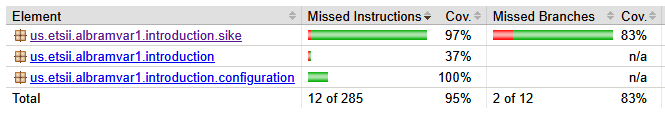
\includegraphics[width=0.85\linewidth]{img/cobertura-modulos.png}
    \caption{Cobertura del proyecto}
    \label{fig:cobertura-modulos}
\end{figure}

Como vemos, la cobertura del módulo 'sike', el que tiene las funcionalidades de generación de claves y cifrado, es de un 97\%, lo que supera el 80\% recomendado.

\begin{figure}[!ht]
    \centering
    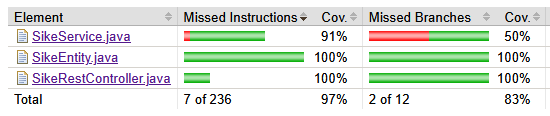
\includegraphics[width=0.75\linewidth]{img/cobertura-clases.png}
    \caption{Cobertura de las clases implementadas}
    \label{fig:cobertura-clases}
\end{figure}

En esta imagen vemos que tanto el controlador como la implementación de la entidad están cubiertas al completo, es sólo el servicio el que no llega al 100\%. Sin embargo, estas líneas no cubiertas son controles explícitos que se han añadido para asegurar el buen funcionamiento interno de la aplicación.

\begin{figure}[!ht]
    \centering
    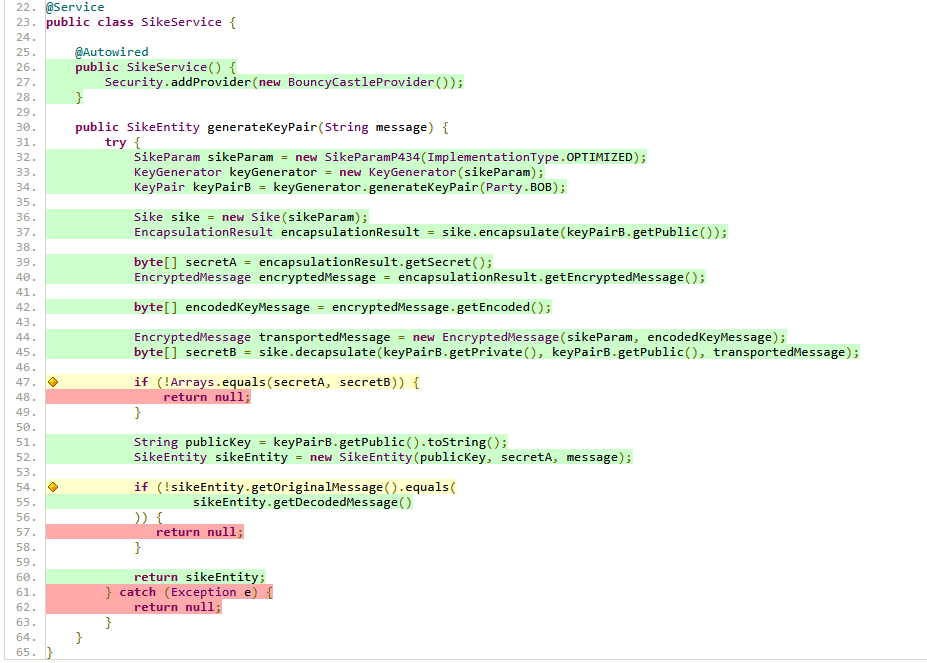
\includegraphics[width=\linewidth]{img/cobertura-servicio.png}
    \caption{Cobertura del servicio}
    \label{fig:cobertura-servicio}
\end{figure}


\section{Frontend}

Aunque el frontend de la aplicación es bastante más grande que el backend, este cumple una función principal de presentación, no teniendo demasiada lógica propia, por lo que obtener una buena cobertura no ha sido difícil.

\subsection{Listado de pruebas}

\begin{longtable}{|p{0.02\linewidth}|p{0.35\linewidth}|p{0.4\linewidth}|p{0.15\linewidth}|}

    % cabecera
    \hline \textbf{Id} & \textbf{Nombre} & \textbf{Descripción} & \textbf{Componente} \\ \hline \endhead
    
    % app
    1 & renders app correctly & Comprueba que que al renderizar la aplicación aparezca la página de inicio. & App \\ \hline

    % about
    2 & renders about section correctly & Comprueba que la sección de información aparezca correctamente. & About \\ \hline
    3 & handle scroll works correctly & Comprueba que la animación de aparición funcione correctamente. & About \\ \hline
    
    % components
    4 & renders message correctly & Comprueba que el mensaje hijo aparezca al renderizar el componente. & AliceToBob \\ \hline
    5 & renders message correctly & Comprueba que el mensaje hijo aparezca al renderizar el componente. & BobToAlice \\ \hline
    6 & renders alice and bob correctly & Comprueba que aparezcan los dos personajes por defecto. & Characters \\ \hline
    7 & hides alice when requested & Comprueba que sólo muestra al personaje deseado, en este caso Bob. & Characters \\ \hline
    8 & hides bob when requested & Comprueba que sólo muestra al personaje deseado, en este caso Alice. & Characters \\ \hline
    9 & renders target text after animation & Comprueba que la animación finaliza con el texto deseado. & DecryptingText \\ \hline
    10 & renders grainient container & Comprueba que el contenedor se renderiza. & Grainient \\ \hline
    11 & renders alice graph view & Comprueba que se renderiza la vista de grafo de Alice por defecto. & GraphView \\ \hline
    12 & renders bob graph view & Comprueba que se renderiza la vista de grafo de Bob cuando se indica. & GraphView \\ \hline
    13 & renders second half correctly & Comprueba que se renderiza la mitad del camino deseado. & GraphView \\ \hline
    14 & load handler is called & Comprueba que el handler ha sido llamado. & GraphView \\ \hline
    15 & renders children with id and classname & Comprueba que los hijos se renderizan correctamente tras la animación. & MotionDiv \\ \hline
    16 & scrolls to top on mount & Comprueba que funciona correctamente al inicio. & ScrollToTop \\ \hline
    17 & renders typewriter container & Comprueba que el contenedor para la animación se renderiza correctamente. & TypewriterText \\ \hline

    % context
    18 & provides initial parameters to children & Comprueba que los valores iniciales se cargan correctamente. & Parameters- Context  \\ \hline

    % footer
    19 & renders footer correctly & Comprueba que el pie de página tiene los componentes necesarios. & Footer \\ \hline

    % hero
    20 & renders hero correctly & Comprueba que la sección hero del inicio contiene a los componentes deseados. & Hero \\ \hline

    % home
    21 & renders home correctly & Comprueba que la página de inicio contiene sus tres componentes principales. & Home \\ \hline

    % navbar
    22 & renders links correctly & Comprueba que la barra de navegación incluye los links necesarios. & Navbar \\ \hline
    23 & home link click & Comprueba la funcionalidad del enlace y la aplicación de estilos. & Navbar \\ \hline
    24 & proof of identity link click & Comprueba la funcionalidad del enlace y la aplicación de estilos. & Navbar \\ \hline
    25 & key exchange link click & Comprueba la funcionalidad del enlace y la aplicación de estilos. & Navbar \\ \hline
    26 & encryption link click & Comprueba la funcionalidad del enlace y la aplicación de estilos. & Navbar \\ \hline
    27 & about link click & Comprueba la funcionalidad del enlace y la aplicación de estilos. & Navbar \\ \hline
    28 & i18n renders in navbar & Comprueba que las opciones de idioma están disponibles en la barra de navegación. & Navbar \\ \hline

    % protocols
    29 & renders protocols correctly & Comprueba que el menú de protocolos aparece correctamente. & Protocols \\ \hline
    30 & handle scroll works correctly & Comprueba que la animación de aparición funciona correctamente. & Protocols \\ \hline

    % protocol view
    31 & renders protocol view correctly & Comprueba que la vista de protocolo contiene los elementos necesarios. & ProtocolView \\ \hline
    32 & renders player correctly & Comprueba que los controles de reproductor aparecen correctamente. & ProtocolView \\ \hline
    33 & player button toggles play & Comprueba que el botón de play inicia la presentación. & ProtocolView \\ \hline
    34 & player button increments and decrements steps & Comprueba el funcionamiento de los controles del reproductor. & ProtocolView \\ \hline
    35 & start button toggles play & Comprueba que el botón de inicio comienza la presentación. & ProtocolView \\ \hline
    36 & renders start controls for proof-of-identity & Comprueba que la vista se renderiza correctamente para el protocolo de prueba de identidad. & ProtocolView \\ \hline
    37 & renders start controls for key-exchange & Comprueba que la vista se renderiza correctamente para el protocolo de intercambio de clave. & ProtocolView \\ \hline
    38 & renders start controls for encryption & Comprueba que la vista se renderiza correctamente para el protocolo de cifrado. & ProtocolView \\ \hline

    % proof of identity
    39 & renders step 1 correctly & Comprueba que el paso se renderiza correctamente. & ProofOfIdentity \\ \hline
    40 & renders step 2 correctly & Comprueba que el paso se renderiza correctamente. & ProofOfIdentity \\ \hline
    41 & renders step 3 correctly & Comprueba que el paso se renderiza correctamente. & ProofOfIdentity \\ \hline
    42 & renders step 4 correctly & Comprueba que el paso se renderiza correctamente. & ProofOfIdentity \\ \hline
    43 & renders step 5 correctly & Comprueba que el paso se renderiza correctamente. & ProofOfIdentity \\ \hline
    44 & step 5 random bit & Comprueba que la animación de bit aleatorio funciona correctamente. & ProofOfIdentity \\ \hline
    45 & renders step 6 correctly & Comprueba que el paso se renderiza correctamente. & ProofOfIdentity \\ \hline

    % key exchange
    46 & renders step 1 correctly & Comprueba que el paso se renderiza correctamente. & KeyExchange \\ \hline
    47 & renders step 2 correctly & Comprueba que el paso se renderiza correctamente. & KeyExchange \\ \hline
    48 & renders step 3 correctly & Comprueba que el paso se renderiza correctamente. & KeyExchange \\ \hline
    49 & renders step 4 correctly & Comprueba que el paso se renderiza correctamente. & KeyExchange \\ \hline
    50 & renders step 5 correctly & Comprueba que el paso se renderiza correctamente. & KeyExchange \\ \hline
    51 & renders step 6 correctly & Comprueba que el paso se renderiza correctamente. & KeyExchange \\ \hline
    52 & renders step 7 correctly & Comprueba que el paso se renderiza correctamente. & KeyExchange \\ \hline

    % encryption
    53 & renders step 1 correctly & Comprueba que el paso se renderiza correctamente. & Encryption \\ \hline
    54 & step 1 handle change & Comprueba que el mensaje se guarda correctamente cuando se escribe en el campo de entrada. & Encryption \\ \hline
    55 & step 1 handle change error & Comprueba que la comprobación de texto funciona correctamente. & Encryption \\ \hline
    56 & renders step 2 correctly & Comprueba que el paso se renderiza correctamente. & Encryption \\ \hline
    57 & step 2 on click & Comprueba que al hacer click se llama al backend. & Encryption \\ \hline
    58 & renders step 3 correctly & Comprueba que el paso se renderiza correctamente. & Encryption \\ \hline
    59 & renders step 4 correctly & Comprueba que el paso se renderiza correctamente. & Encryption \\ \hline
    60 & renders step 5 correctly & Comprueba que el paso se renderiza correctamente. & Encryption \\ \hline
    61 & renders step 6 correctly & Comprueba que el paso se renderiza correctamente. & Encryption \\ \hline
    
    \caption{Listado completo de tests del frontend}
    \label{tab:tests-frontend}
\end{longtable}


\subsection{Cobertura}

La cobertura obtenida con estos tests ha sido bastante buena, aunque no perfecta. En total ha sido de casi un 90\%, y la mitad exacta (seis de los 12 componentes cuya cobertura se comprueba) tienen una cobertura del 100\%.

Hay dos componentes en concreto que tienen una cobertura nula y estos son el index.js y el i18n.js. Esta falta de cobertura se debe a desconocimiento de cómo diseñar una suite de tests orientada a ellos además de un testing informal que se ha realizado a lo largo del desarrollo y también justo antes de hacer cualquier subida.

En la siguiente página se incluye el desglose completo de la cobertura obtenida.

\begin{figure}[!ht]
    \centering
    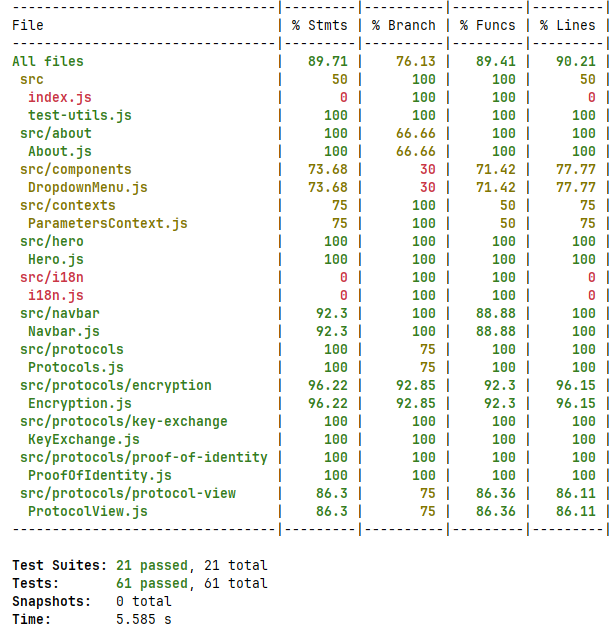
\includegraphics[width=\linewidth]{img/cobertura-frontend.png}
    \caption{Cobertura obtenida}
    \label{fig:cobertura-frontend}
\end{figure}
     \chapter{Desarrollo}\label{desarrollo}

\section{Incidencias}

Como todo desarrollo software, el proceso de creación de la interfaz ha tenido varias incidencias que quedarán registradas en esta sección.

\subsection{Despliegue en Render}

Como mencionamos en el capítulo \ref{tecnologias} Tecnologías, tras un proceso de investigación y selección acabamos decidiendo desplegar en Render. A pesar de ser una herramienta que conocemos y con la que hemos trabajado anteriormente, nos hemos encontrado con algunos problemas.

El principal entre ellos es la disponibilidad del despliegue. Render suspende aquellos servicios que no reciben ninguna petición tras 15 minutos. Para evitar esto, utilizamos UptimeRobot, un servicio web que cada cierto tiempo (en este caso concreto, 5 minutos) consulta la página para evitar que Render la suspenda.

Sin embargo, esta no es la única restricción que Render aplica a sus despliegues gratuitos, también aplica un máximo de 750 horas de disponibilidad. Lo que es más que suficiente para un proyecto como este, aunque no equivale a las 24 horas de los 31 días del mes. Por este motivo, el servicio quedó suspendido del 27 de mayo hasta el 31 de ese mismo mes. Para evitar estos periodos de no disponibilidad, tuvimos que investigar por otro servicio gratuito similar a UptimeRobot pero que incluyese periodos de mantenimiento, lo que permitiría reducir el número de horas que el servicio está disponible.

La mayoría de servicios de monitorización web que incluyen intervalos de mantenimiento son de pago (el servicio en sí no necesariamente, pero esa funcionalidad sí) pero tras mucho buscar dimos con Better Stack, que incluye esta funcionalidad de manera gratuita. Establecemos así un periodo de mantenimiento diario desde las 12 de la noche hasta las 6 de la mañana, permitiendo así que el despliegue se suspenda durante esas horas y consiguiendo así no llegar a las 750 horas de disponibilidad que Render ofrece.



\section{Desarrollos futuros}

En esta sección se discutirán los posibles desarrollos que podrían incluirse en la interfaz pero que no ha sido posible incluirlos en el despligue actual.

\subsection{Apartado de conceptos matemáticos}

Aunque la interfaz no profundiza mucho en el funcionamiento matemático del protocolo, podría ser interesante incluir aquellos conceptos que se discuten en esta memoria en el capítulo \ref{conceptosprevios} titulado Conceptos previos.

Esta página podría reutilizar la plantilla de protocolo o bien ser una página simple al estilo Wikipedia donde se concentre la información. En esta segunda opción, cada sección podría ocultarse o mostrarse con una animación tipo acordeón que permitiese moverse libre y fácilmente por todo el documento.

Esta funcionalidad no ha sido incluida por no disponer del tiempo de realizarla correctamente.


\subsection{Ampliación de los workflows}

Aunque la interfaz es un proyecto pequeño, podría ser interesante incluir algunas funcionalidades a los workflows existentes.

Ahora mismo, el despliegue lo dirige Render, si los workflows básicos de pruebas pasan y el commit incluye cambios en un directorio determinado (dado que tenemos tanto frontend como backend en un mismo repositorio, esta especificación permite no hacer despliegues innecesarios). Sin embargo, podría ser interesante incluir el despliegue en el mismo workflow.

También, como los despliegues se realizan mediante Docker, podría ser interesante incluir una publicación de la imagen o similar.

Siguiendo la lógica de la comprobación de las pruebas, podría incluirse un servicio como son Codacy o Sonarqube que permiten un análisis del código y su calidad.

Estos desarrollos no se han realizado debido al pequeño tamaño del proyecto.


\subsection{Personalizar y/o dinamizar la presentación del intercambio de clave}

Igual que el protocolo de cifrado es dinámico, cifrando y descifrando el mensaje que introduce el usuario utilizando SIKE, la presentación de intercambio de clave podría permitir al usuario la elección de primo y parámetros iniciales para que cada experiencia sea diferente y el usuario pueda apreciar las diferencias entre la aplicación de unos parámetros u otros.

Sin embargo, permitir tanta variabilidad haría que el proyecto se saliese del alcance, el tiempo y los recursos disponibles. No tenemos los conocimientos necesarios para implementar unos desarrollos matemáticos tan complejos y, aunque investigando habríamos podido llegar a obtenerlos, este proceso de investigación se saldría de los plazos disponibles. 


\subsection{Prueba de conocimiento cero}

La propuesta del SIKE al NIST incluye también una prueba de conocimiento cero. Este protocolo también estuvo originalmente incluido en el proyecto (de hecho, sigue presente en la interfaz gráfica) pero finalmente, por consejo del tutor, decidimos eliminarlo y considerarlo como una posible mejora futura.
     \chapter{Conclusiones}\label{conclusiones}

El principal objetivo de este proyecto es acercar el protocolo diseñado por de Feo, Jao y Plût a una persona con un leve conocimiento de criptografía. Para ello, hemos realizado una investigación sobre las bases matemáticas del protocolo que después hemos simplificado en el capítulo \ref{conceptosprevios} titulado Conceptos previos. Esta investigación ha sido extensa, ya que para entender íntegramente la extensa base que tiene SIKE hemos dado, a lo mejor, unos cuantos rodeos de más. No obstante, estos han sido finalmente necesarios para determinar qué conceptos eran realmente importantes por sus implicaciones y cuales no.

Naturalmente, este trabajo incluye también la redacción y revisión continua de los capítulos didácticos que son el capítulo \ref{conceptosprevios}  ya mencionado así como el capítulo \ref{estudioteorico} titulado Estudio teórico. 

De manera paralela se ha realizado una implementación gráfica que a nivel de interfaz refleja lo redactado en el capítulo \ref{estudioteorico} y a nivel de código ejemplifica cómo utilizar la implementación de SIKE en Java.

En nuestras investigaciones, tanto sobre el protocolo en sí como búsquedas técnicas específicas de problemas de desarrollo, sólo hemos encontrado un otro trabajo parecido a este. Se trata de una tesis equivalente a un trabajo fin de grado titulado \textit{Implementation of SIKE in Java: A detailed and comprehensive guide for understanding and implementing SIKE - A NIST Post-Quantum-Competition candidate} \cite{sike-implementation}. En cambio, este trabajo se centra en buscar una optimización de SIKE. Se desarrolla una implementación original de SIDH en SageMath y una de SIDH/SIKE en Java y, aunque explica las funciones más importantes, lo hace de manera formal. Este trabajo por Schubert no está pensado para iniciar a alguien a SIKE sino a desarrollar SIKE como protocolo.

En relación al desarrollo del proyecto, me siento orgullosa de la labor de investigación realizada. Se tratan temas difíciles y aunque ha habido veces que he sentido que estaba entrando en una agujero de conejo, una vez terminado he disfrutado la experiencia de desmigar un problema, encontrar las bases y construir mi propio conocimiento a partir de ahí.

De igual manera, el desarrollo de la interfaz ha sido bastante manual. Acostumbrada a empezar de una plantilla para todo proyecto que hemos realizado en clase (por motivos de tiempo y comodidad, principalmente) me propuse hacer este proyecto, entender realmente como se conecta todo. Hoy en día que la inteligencia artificial parece ser capaz de hacerlo todo en segundos, he querido centrarme en las bases que nunca antes había aprendido, 

Como he mencionado, el desarrollo es casi íntegramente personal. Usando la inteligencia artificial (el agente por defecto de Cursor) para corregir los fallos del entorno de pruebas del frontend, ya que llevaba días intentando configurarlo pero no conseguía que se llegasen siquiera a ejecutar. El resto des trabajo, investigación, redacción y desarrollo, es propio.

Este trabajo ha avanzado más lento de lo que tenía previsto, debido a la complejidad de las matemáticas pero también por cuestiones personales. Aun así, estoy contenta con el trabajo realizado. Habiendo empezado el doble grado en matemáticas e informática, decidí hacer este TFG, probablemente más matemático de lo normal en esta carrera, por volver a acercarme a esta disciplina. 

\backmatter

\bibliographystyle{apacite}
\bibliography{pfcbib}

\end{document}
